\documentclass[10pt]{beamer}
\usetheme[
%%% options passed to the outer theme
%    progressstyle=fixedCircCnt,   %either fixedCircCnt, movCircCnt, or corner
%    rotationcw,          % change the rotation direction from counter-clockwise to clockwise
%    shownavsym          % show the navigation symbols
  ]{AAUsimple}

% If you want to change the colors of the various elements in the theme, edit and uncomment the following lines
% Change the bar and sidebar colors:
%\setbeamercolor{AAUsimple}{fg=red!20,bg=red}
%\setbeamercolor{sidebar}{bg=red!20}
% Change the color of the structural elements:
%\setbeamercolor{structure}{fg=red}
% Change the frame title text color:
%\setbeamercolor{frametitle}{fg=blue}
% Change the normal text color background:
%\setbeamercolor{normal text}{fg=black,bg=gray!10}
% ... and you can of course change a lot more - see the beamer user manual.

\usepackage[utf8]{inputenc}
\usepackage[english]{babel}
\usepackage[T1]{fontenc}
\usepackage{mathenv}
\usepackage{empheq}
\usepackage{subfigure}
\usepackage{multimedia}
\usepackage{pgf,tikz}
\usetikzlibrary{positioning,arrows}
%\usepackage[pdftex]{hyperref}
\usepackage{mathrsfs}
\usepackage{mathtools}
\mathtoolsset{showonlyrefs=true}

\usepackage{multicol}
\usepackage{empheq}
\usepackage{textpos}
\usepackage{graphics}
% Or whatever. Note that the encoding and the font should match. If T1
% does not look nice, try deleting the line with the fontenc.
\usepackage{helvet}
\usepackage{tikz,pgfplots,xcolor}

\pgfplotsset{compat=newest}

%%%%%% TIKZ SET STYLE %%%%%%%%
\tikzset{boxOptions/.style={
    rectangle,
    rounded corners,
    draw=black, very thick,
    text width=9em,
    minimum height=2em,
    text centered}
}

\tikzset{arrowStyle/.style={
    ->,
    thick,
    shorten <=2pt,
    shorten >=2pt}
}

\tikzset{arrowStyleinv/.style={
    <-,
    thick,
    shorten <=2pt,
    shorten >=2pt}
}

\usetikzlibrary{backgrounds}

\newcommand\tikzscale{0cm}
\newlength{\tikzwidth}
\newlength{\tikzheight}

%%%%%%%%%%%%%%%%%%%%%%%%%%%%

% colored hyperlinks
\newcommand{\chref}[2]{%
  \href{#1}{{\usebeamercolor[bg]{AAUsimple}#2}}%
}
\newcommand{\scaption}[1]{\caption{\tiny{#1}}}


\definecolor{light-gray}{gray}{0.95}
\definecolor{myred}{RGB}{200,0,0}
\newcommand{\myred}{red!70!black}
\newcommand{\mygreen}{green!60!black}
\newcommand{\myblue}{blue!40!black}
\newcommand{\code}[1]{\colorbox{light-gray}{\texttt{#1}}}


\newcommand\discreteP{\boldsymbol{\textcolor{\myred}{\bar{P}}}}
\newcommand\discreteV{\boldsymbol{\textcolor{\myred}{\bar{V}}}}
\newcommand\discreteU{\boldsymbol{\textcolor{\myred}{\bar{U}}}}
\newcommand\discreteF{\boldsymbol{\bar{F}}}
\newcommand\discreteG{\boldsymbol{\bar{G}}}

\newcommand\discreteQP{\bar{q_p}}
\newcommand\discreteQV{\bar{q_v}}
\newcommand\discreteQ{\bar{q}}
%\newcommand\discreteD{\bar{d}}
\newcommand\Lag{\mathcal{L}}

\newcommand\contP{\boldsymbol{\textcolor{\myred}{p}}}
\newcommand\contV{\boldsymbol{\textcolor{\myred}{v}}}
%\newcommand\contP{p}
%\newcommand\contV{\textbf{v}}
%\newcommand\contV{v}
\newcommand\contU{\textbf{u}}
\newcommand\qcqU{\widehat{\textbf{u}}}
\newcommand\qcqP{\widehat{p}}
\newcommand\qcqV{\widehat{\textbf{v}}}
\newcommand\contLbd{\boldsymbol{\lambda}}
\newcommand\qcqLbd{\boldsymbol{\widehat{\lambda}}}
\newcommand\Lbdun{\boldsymbol{\textcolor{\myred}{\lambda_1}}}
\newcommand\Lbdeux{\boldsymbol{\textcolor{\myred}{\lambda_2}}}
\newcommand\qcqLbdun{\widehat{\lambda_1}}
\newcommand\qcqLbdeux{\boldsymbol{\widehat{\lambda_2}}}

\newcommand\discreteLbd{\textcolor{\myred}{\boldsymbol{\bar{\Lambda}}}}
\newcommand\discreteLbdun{\textcolor{\myred}{\boldsymbol{\bar{\Lambda_1}}}}
\newcommand\discreteLbdeux{\textcolor{\myred}{\boldsymbol{\bar{\Lambda_2}}}}
\newcommand\discreteD{\boldsymbol{\bar{D}}}

\newcommand\CF{\mathcal{J}}

\newcommand\contAl{\boldsymbol{\alpha}}
\newcommand\normal{\boldsymbol{n}}

%% \newcommand\velocity{v_p}
%% \newcommand\density{\rho_0}
\newcommand\velocity{\boldsymbol{\textcolor{\mygreen}{c}}}
\newcommand\bulkmodulus{\boldsymbol{\textcolor{\mygreen}{\kappa}}}
\newcommand\density{\boldsymbol{\textcolor{\mygreen}{\rho}}}

\newcommand{\modelfile}{blabla.png}

\pgfplotsset{
        colormap/paraview/.style={
                colormap={paraview}{
                        rgb255(0cm)=(20,119,255)
			rgb255(1cm)=(168,181,255)
			rgb255(2cm)=(240,240,240)
			rgb255(3cm)=(255,161,145)
                        rgb255(4cm)=(234,60,53)
                },
        },
}

\newlength{\plotwidth}
\newlength{\plotheight}
\setlength{\plotwidth} {6cm}
\setlength{\plotheight}{7cm}



\newcommand\vectll[4]{\left#1 \begin{array}{c}
    #2\\
    #3\\
  \end{array} \right#4}



\title[\textbf{Time Domain FWI involving DG approximation}]{\textbf{Time Domain Full Waveform Inversion \\  involving Discontinuous Galerkin \\ approximation}}


\AtBeginSection[]
{  \frame<handout:0>
  {    \frametitle{Outline}
    \tableofcontents[sectionstyle=show/shaded,
           subsectionstyle=show/shaded/shaded]
  }
}
\renewcommand{\thesubfigure}{\relax}
%\subtitle{v.\ 1.2.1}  % could also be a conference name

\date{\textbf{Waves 2019}}

\author{
  \textbf{Pierre Jacquet}\\
  \href{mailto:pierre.jacquet@inria.fr}{{\tt pierre.jacquet@inria.fr}}
}

% - Give the names in the same order as they appear in the paper.
% - Use the \inst{?} command only if the authors have different
%   affiliation. See the beamer manual for an example

\institute[
%  {\includegraphics[scale=0.2]{aau_segl}}\\ %insert a company, department or university logo
 \textbf{ First year PhD Student\\
  Inria - Magique 3D - DIP\\
  Pau, FRANCE}
] % optional - is placed in the bottom of the sidebar on every slide
{% is placed on the bottom of the title page
  \textbf{ Barucq Hélène, Diaz Julien, Calandra Henri \\
    First year PhD Student\\
   Inria - Magique 3D - DIP\\
  Pau, FRANCE}
  %there must be an empty line above this line - otherwise some unwanted space is added between the university and the country (I do not know why;( )
}

% specify a logo on the titlepage (you can specify additional logos an include them in
% institute command below
\pgfdeclareimage[height=2cm]{titlepagelogo}{AAUgraphics/bandeau.png} % placed on the title page
%\pgfdeclareimage[height=1.5cm]{titlepagelogo2}{AAUgraphics/aau_logo_new} % placed on the title page
\titlegraphic{% is placed on the bottom of the title page
  \pgfuseimage{titlepagelogo}
%  \hspace{1cm}\pgfuseimage{titlepagelogo2}
}

\begin{document}
% the titlepage
{\aauwavesbg%
\begin{frame}[plain,noframenumbering] % the plain option removes the header from the title page
  \titlepage
\end{frame}}
%%%%%%%%%%%%%%%%

% TOC
%% \begin{frame}{Outline}{}
%% \tableofcontents
%% \end{frame}
%%%%%%%%%%%%%%%%

%{
  \AtBeginSection[]{}
  \section{Time Domain Full Waveform Inversion}
}

\subsection{Seismic Acquisition}

% ============================================
% ====== Frame : Seismic Acquisition  ========
% ============================================
\begin{frame}{Seismic Acquisition}


  \begin{figure}
    \def\svgwidth{1.05\linewidth}
    \input{images/intro_1.pdf_tex}
  \end{figure}

\end{frame}

\begin{frame}[noframenumbering]{Seismic Acquisition}


  \begin{figure}
    \def\svgwidth{1.05\linewidth}
    \input{images/intro_2.pdf_tex}
  \end{figure}

\end{frame}

\newcommand\hideit[1]{%
  \only<0| handout:1>{\mbox{}}%
  \invisible<0| handout:1>{#1}}







% ============================================
% ====== Frame : FWI Workflow 1       ========
% ============================================
\subsection{FWI Workflow}

\begin{frame}{FWI Workflow}
  \begin{columns}
    \column{\dimexpr\paperwidth-10pt}
    \begin{figure}
      \def\svgwidth{1.0\linewidth}
      \input{images/data.pdf_tex}
    \end{figure}
  \end{columns}
  \vspace{4.5cm}
~
\end{frame}

\begin{frame}[noframenumbering]{FWI Workflow}
  \begin{columns}
    \column{\dimexpr\paperwidth-10pt}
    \begin{figure}
      \def\svgwidth{1.0\linewidth}
      \input{images/data_2.pdf_tex}
    \end{figure}
  \end{columns}
  \vspace{1cm}
  \uncover<2->{
    Cost function to minimize :
    \begin{equation}
      \CF(\model) = \frac{1}{2}||\textcolor{blue}{d_{obs}}-\textcolor{red}{\mathcal{F}(\model)}||^2dt
    \end{equation}
 \begin{itemize}
   \item $\mathcal{F}(m)$ is the restriction on the receivers of the simulated waves in the media $\model$. (With $\model = \velocity, \density, \bulkmodulus$...)
   \item FWI iterates until $\CF(\model) \longrightarrow 0$
 \end{itemize}
  }
\end{frame}






% ============================================
% ====== Frame : FWI Workflow 2       ========
% ============================================

\begin{frame}{FWI Workflow}
\begin{figure}
  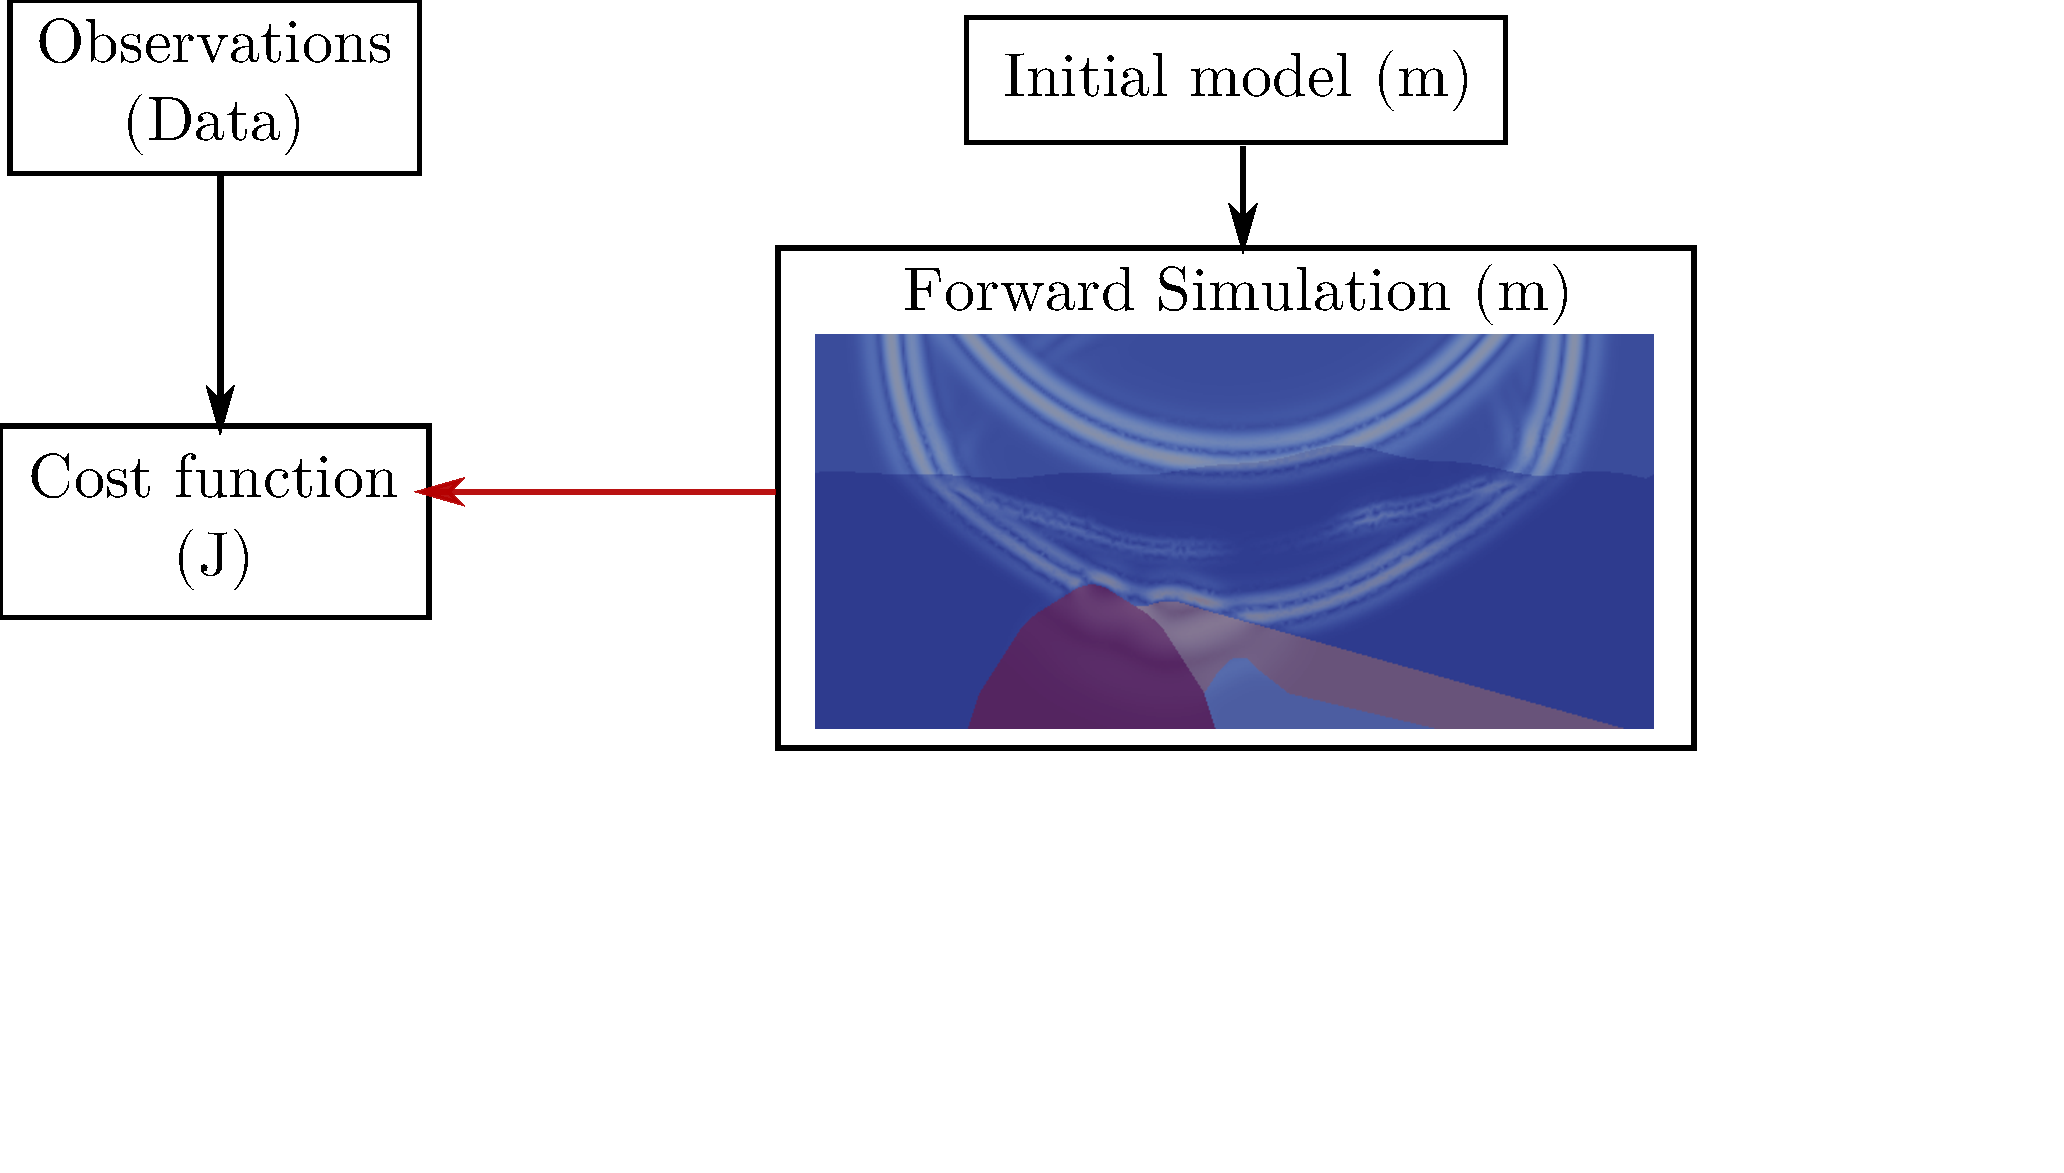
\includegraphics[scale=0.31]{fwi_test1.pdf}
\end{figure}
\end{frame}

\begin{frame}[noframenumbering]{FWI Workflow}
\begin{figure}
  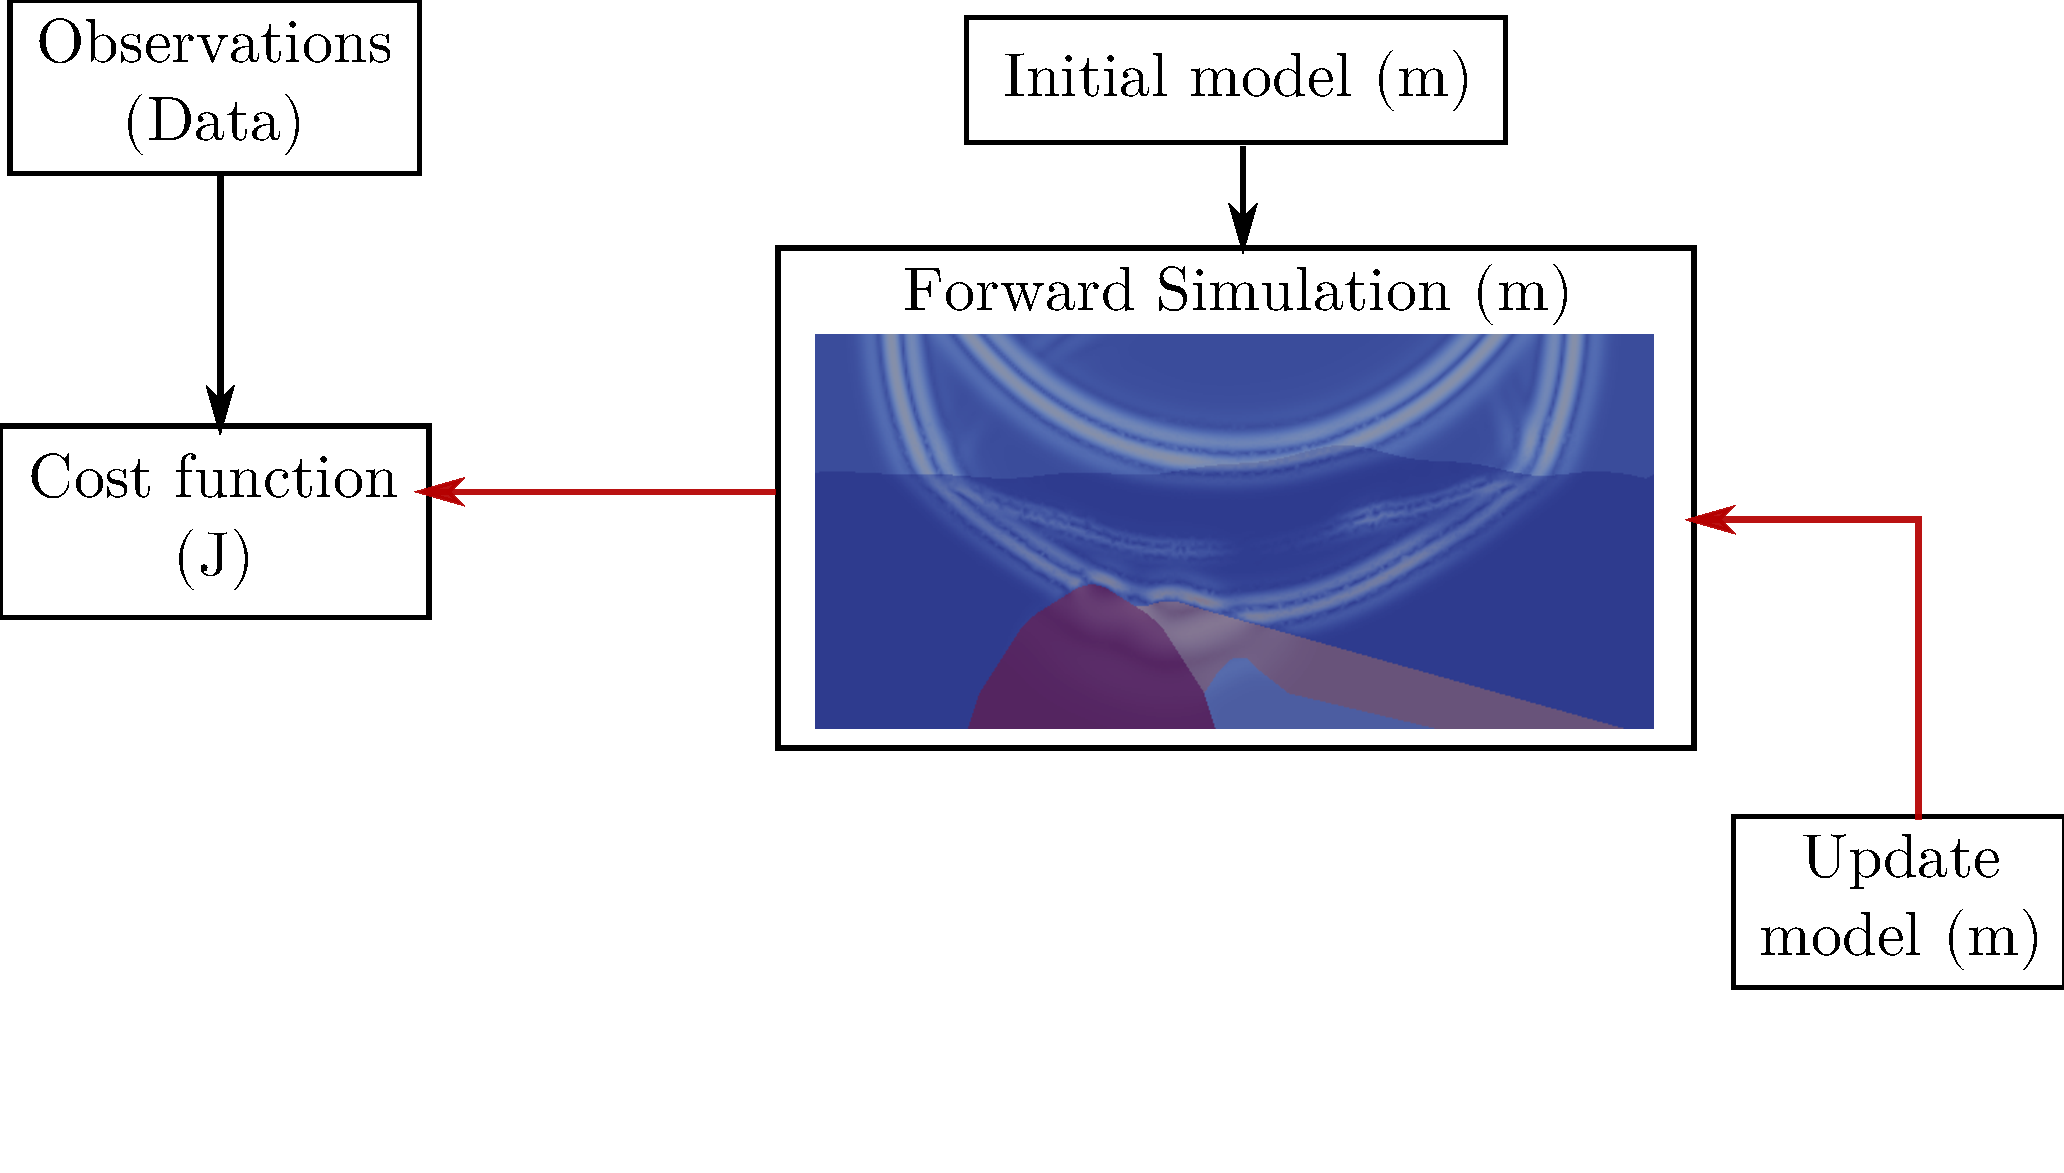
\includegraphics[scale=0.31]{fwi_test2.pdf}
\end{figure}
\end{frame}


\begin{frame}[noframenumbering]{FWI Workflow}
\begin{figure}
  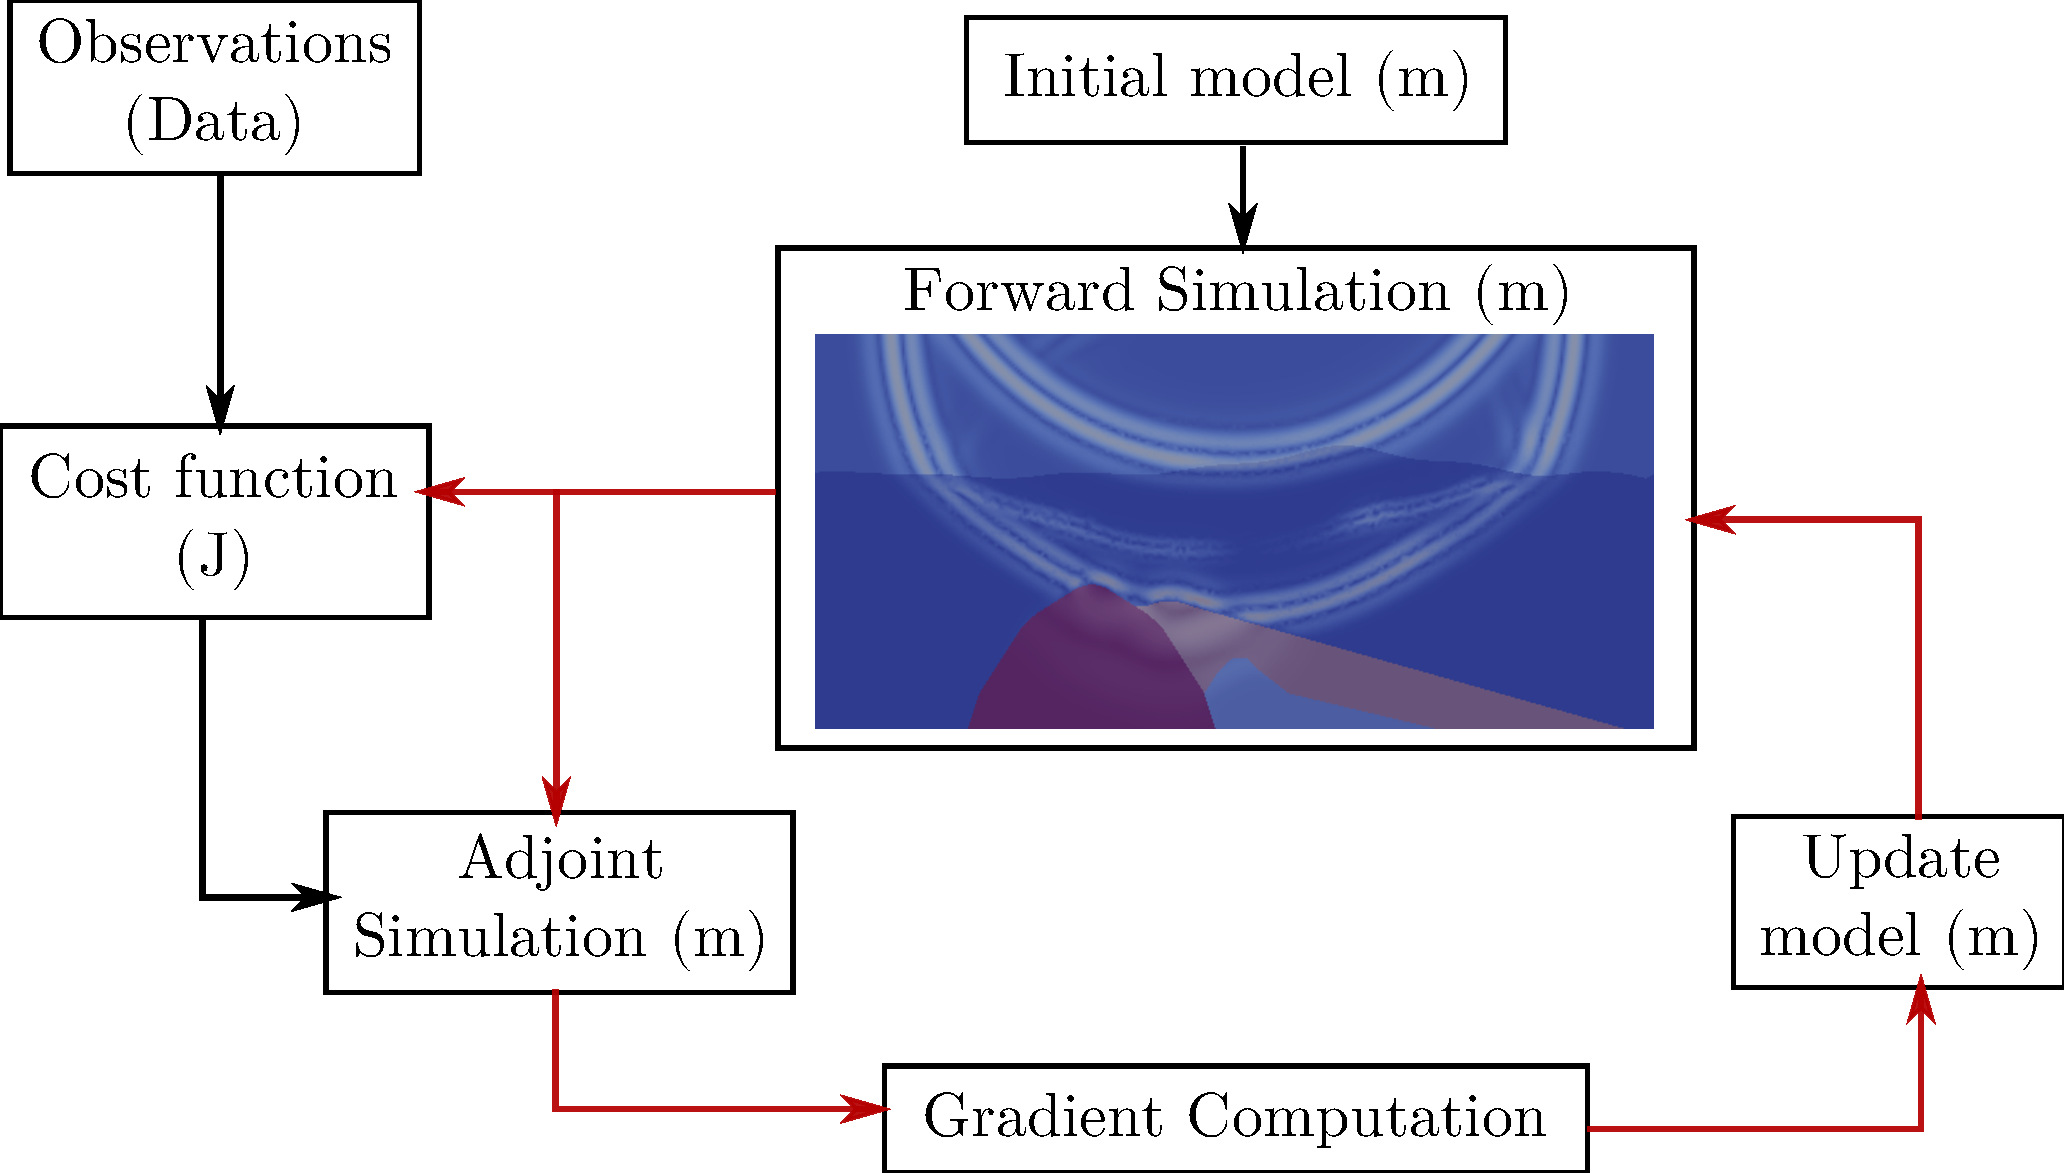
\includegraphics[scale=0.31]{fwi_test.pdf}
\end{figure}
\end{frame}

\begin{frame}[noframenumbering]{FWI Workflow}
\begin{figure}
  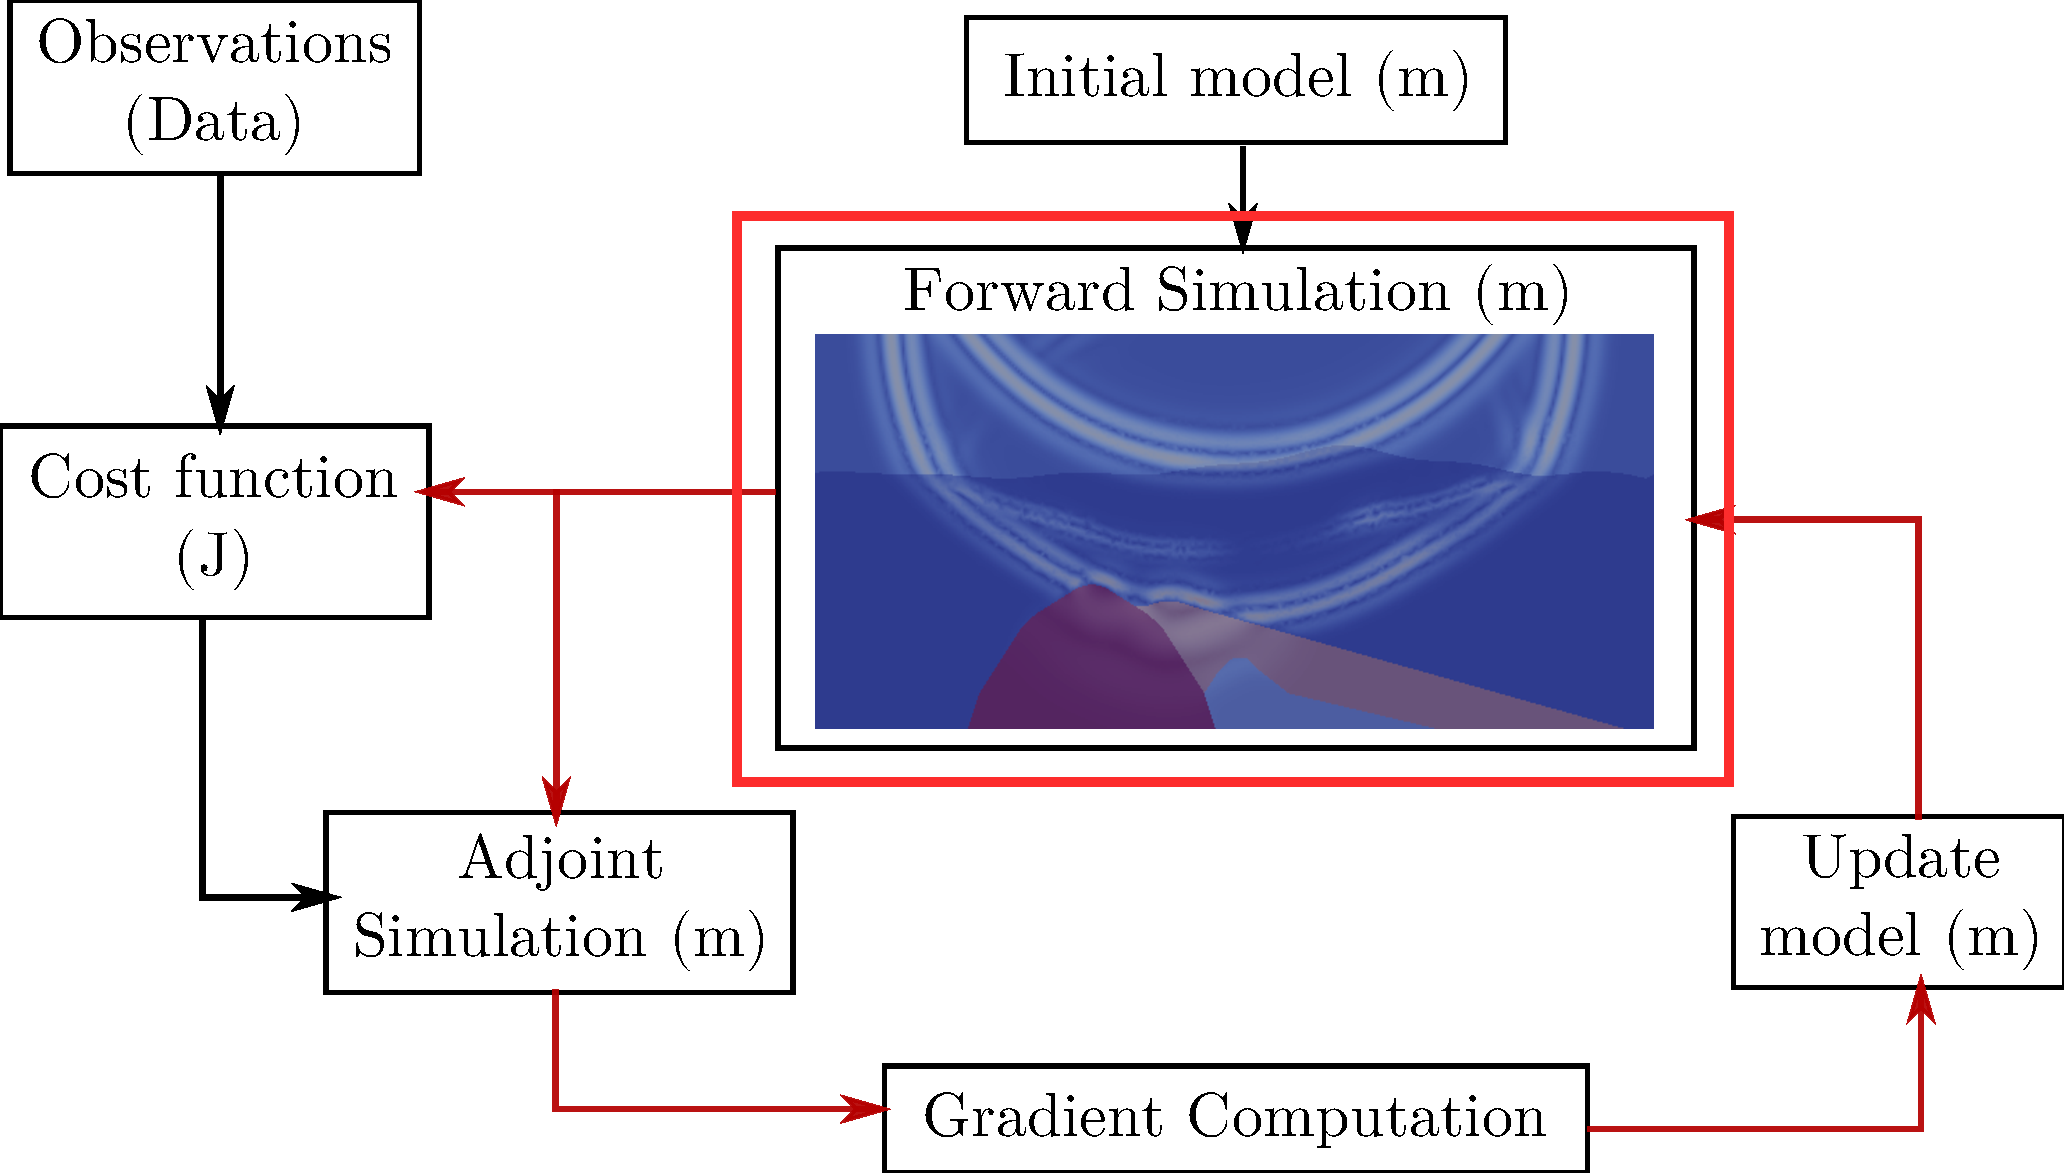
\includegraphics[scale=0.31]{fwi_test3.pdf}
\end{figure}
\end{frame}



% ============================================
% ====== Frame : Forward Continuous Model ====
% ============================================

\subsection{Forward Discretization}
\begin{frame}{Continuous Forward Model}

  First order acoustic wave equation
  \begin{multicols}{2}
  \begin{empheq}[left=\empheqlbrace]{align}
    & \frac{1}{\density \velocity^2}\frac{\partial \contP}{\partial t}+\nabla \cdot \contV=f_p \text{~~ on $\boldsymbol{\Omega}$}\\
    & \density\frac{\partial \contV}{\partial t}+\nabla\contP=0  \text{~~ on $\boldsymbol{\Omega}$}\\
    & \contP=0 \text{~~ on $\textcolor{red}{\boldsymbol{\Gamma_1}}$} \\
    & \frac{\partial \contP}{\partial t}+\velocity \nabla \contP \cdot \normal=0 \text{~~ on $\textcolor{blue}{\boldsymbol{\Gamma_2}}$}
  \end{empheq}

  \columnbreak

  \begin{center}
    \renewcommand\tikzscale{1.0}
    \begin{figure}[H]
    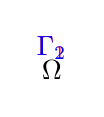
\begin{tikzpicture}[scale=\tikzscale]
\draw[color=blue,line width=2,double] (0,0) -- (5,0);
\draw[color=blue,line width=2,double] (0.07,-0.07) -- (0.07,3);
\draw[color=blue,line width=2,double] (4.93,-0.07) -- (4.93,3);
\draw[color=red,line width=2.1](-0.,3) -- (5,3);


\node[anchor=south, color=red]
at (2.5,3) {$\Gamma_1$};

\node[anchor=south, color=blue]
at (2.5,0) {$\Gamma_2$};

\node[color=black]
at (2.5,1.5) {$\Omega$};
\end{tikzpicture}

    \small{Domain with Absorbing Boundary Conditions}
    \end{figure}
  \end{center}

  \end{multicols}
\end{frame}





% ============================================
% ====== Frame : Forward Discrete Model ======
% ============================================

\begin{frame}{Discrete Forward Model}

  \begin{multicols}{2}

    Space Discretization : Discontinuous Galerkin Elements
    \begin{itemize}
      \item Nodal \small{(Lagrangian / Jacobian)}
      \item \normalsize{Modal} \small{(Bernstein-Bézier)}
    \end{itemize}
    \vspace{1cm}
    \uncover<3->{
    Time schemes :
    \begin{itemize}
      \item Runge Kutta 2/4
      \item Adams Bashforth 3
    \end{itemize}}

    \columnbreak

    \uncover<2->{
    Semi-discretized model :
    \begin{equation}
      \frac{\partial}{\partial t}\discreteU(t) = A \discreteU(t) + \discreteF(t)
    \end{equation}

    with :

    \begin{equation}
      \discreteU(t)=\vectll{(}{\discreteP(t)}{\discreteV(t)}{)}
    \end{equation}}

    \uncover<3->{
    \begin{figure}
      \noindent
       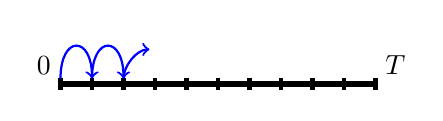
\begin{tikzpicture}[scale=0.8]
      \draw[color=black,line width=2.1](0.0,0.0) -- (5,0.0);
      %\draw[color=blue, line width=10] (0,-0.02) node {$\bullet$} ;
      %\draw[color=blue, line width=10] (5,-0.02) node {$\bullet$} ;
     % \draw node[color=blue,fill,circle,minimum size=0.01](1,1) {};
      \node[anchor=south east, color=black]
      at (0,0) {$0$};
      \node[anchor=south west, color=black]
      at (5,0) {$T$};
      
      \pgfmathsetmacro{\x}{0.0}
      \draw[color=black,line width=2.1](\x,0.1) -- (\x,-0.1);

      \pgfmathsetmacro{\x}{5.0}
      \draw[color=black,line width=2.1](\x,0.1) -- (\x,-0.1);

      \pgfmathsetmacro{\x}{0.5}
      \draw[color=black,line width=1.5](\x,0.1) -- (\x,-0.1);
      \draw[arrowStyle,color=blue]
      (\x-0.5,0) to[out=90,in=90,looseness=4.0]
      node[sloped,anchor=south]
      {}
      (\x,0.0);
      \draw[color=black,line width=1.5](\x,0.1) -- (\x,-0.1);


      
      \pgfmathsetmacro{\x}{1.0}
            \draw[arrowStyle,color=blue]
      (\x-0.5,0) to[out=90,in=90,looseness=4.0]
      node[sloped,anchor=south]
      {}
      (\x,0.0);
      \draw[color=black,line width=1.5](\x,0.1) -- (\x,-0.1);
      \pgfmathsetmacro{\x}{1.5}
            \draw[arrowStyle,color=blue]
      (\x-0.5,0) to[out=90,in=180,looseness=1.0]
      node[sloped,anchor=south]
      {}
      (\x,0.55);

      
      \draw[color=black,line width=1.5](\x,0.1) -- (\x,-0.1);
      \pgfmathsetmacro{\x}{2.0}
      \draw[color=black,line width=1.5](\x,0.1) -- (\x,-0.1);
      \pgfmathsetmacro{\x}{2.5}
      \draw[color=black,line width=1.5](\x,0.1) -- (\x,-0.1);
      \pgfmathsetmacro{\x}{3.0}
      \draw[color=black,line width=1.5](\x,0.1) -- (\x,-0.1);
      \pgfmathsetmacro{\x}{3.5}
      \draw[color=black,line width=1.5](\x,0.1) -- (\x,-0.1);
      \pgfmathsetmacro{\x}{4.0}
      \draw[color=black,line width=1.5](\x,0.1) -- (\x,-0.1);
      \pgfmathsetmacro{\x}{4.5}
      \draw[color=black,line width=1.5](\x,0.1) -- (\x,-0.1);
    \end{tikzpicture}

      Forward time steps
    \end{figure}}

  \end{multicols}

\end{frame}






% ============================================
% ====== Frame : Asset of DGs  ===============
% ============================================

\begin{frame}{Discrete Forward Model}{Discontinuous Galerkin Method}
  Asset of Discontinuous Galerkin Methods : \\

  \begin{itemize}
  \item Unstructured grid (enable to match the topography and media irregularities)
  \item Robust to physical discontinuities
  \item hp-adaptivity
  \item Massively parallel performance properties
  \end{itemize}

  \begin{figure}[H]
    \centering
    \subfigure[h-adaptivity]{
      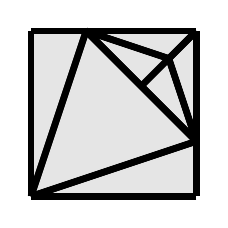
\begin{tikzpicture}[scale=0.7]%[line cap=round,line join=round,>=triangle 45,x=1.0cm,y=1.0cm]
      %% \draw[->,color=black] (-1.05,0) -- (9.66,0);
      %% \foreach \x in {-1,-0.5,0.5,1,1.5,2,2.5,3,3.5,4,4.5,5,5.5,6,6.5,7,7.5,8,8.5,9,9.5}
      %% \draw[shift={(\x,0)},color=black] (0pt,2pt) -- (0pt,-2pt) node[below] {\footnotesize $\x$};
      %% \draw[->,color=black] (0,-0.43) -- (0,5.53);
      %% \foreach \y in {,0.5,1,1.5,2,2.5,3,3.5,4,4.5,5,5.5}
      %% \draw[shift={(0,\y)},color=black] (2pt,0pt) -- (-2pt,0pt) node[left] {\footnotesize $\y$};
      %% \draw[color=black] (0pt,-10pt) node[right] {\footnotesize $0$};
      %% \clip(-1.05,-0.43) rectangle (9.66,5.53);
      \fill[line width=2.4pt,fill=black,fill opacity=0.1] (1,1) -- (4,2) -- (4,1) -- cycle;
      \fill[line width=2.4pt,fill=black,fill opacity=0.1] (1,1) -- (1,4) -- (2,4) -- cycle;
      \fill[line width=2.4pt,fill=black,fill opacity=0.1] (2,4) -- (4,2) -- (1,1) -- cycle;
      \fill[line width=2.4pt,fill=black,fill opacity=0.1] (2,4) -- (4,4) -- (4,2) -- cycle;
      \draw [line width=2.4pt] (1,1)-- (4,2);
      \draw [line width=2.4pt] (4,2)-- (4,1);
      \draw [line width=2.4pt] (4,1)-- (1,1);
      \draw [line width=2.4pt] (1,1)-- (1,4);
      \draw [line width=2.4pt] (1,4)-- (2,4);
      \draw [line width=2.4pt] (2,4)-- (1,1);
      \draw [line width=2.4pt] (2,4)-- (4,2);
      \draw [line width=2.4pt] (4,2)-- (1,1);
      \draw [line width=2.4pt] (1,1)-- (2,4);
      \draw [line width=2.4pt] (2,4)-- (4,4);
      \draw [line width=2.4pt] (4,4)-- (4,2);
      \draw [line width=2.4pt] (4,2)-- (2,4);
      \draw [line width=2.4pt] (2,4)-- (3.5,3.5);
      \draw [line width=2.4pt] (3,3)-- (4,4);
      \draw [line width=2.4pt] (4,4)-- (2,4);
      \draw [line width=2.4pt] (2,4)-- (3.5,3.5);
      \draw [line width=2.4pt] (3.5,3.5)-- (4,2);
      \draw [line width=2.4pt] (4,2)-- (2,4);
      \draw [line width=2.4pt] (4,2)-- (4,4);
      \draw [line width=2.4pt] (4,4)-- (3.5,3.5);
      \draw [line width=2.4pt] (3.5,3.5)-- (4,2);
  \end{tikzpicture}

}
    \hspace{1cm}
  \subfigure[p-adaptivity with \textcolor{black}{P1}, \textcolor{blue}{P2}, \textcolor{red}{P3} elements]{
      \definecolor{ccqqqq}{rgb}{0.8,0,0}
    \definecolor{qqqqff}{rgb}{0,0,1}
    \definecolor{cccccc}{rgb}{0.8,0.8,0.8}
    \begin{tikzpicture}[scale=0.7]
      %\draw[->,color=black] (0,0.62) -- (0,4.91);
      %\foreach \y in {0.6,0.8,1,1.2,1.4,1.6,1.8,2,2.2,2.4,2.6,2.8,3,3.2,3.4,3.6,3.8,4,4.2,4.4,4.6,4.8}
      %\draw[shift={(0,\y)},color=black] (2pt,0pt) -- (-2pt,0pt) node[left] {\footnotesize $\y$};
      %\clip(-0.64,0.62) rectangle (7.09,4.91);
      \fill[line width=1.6pt,color=cccccc,fill=cccccc,fill opacity=0.15] (1,1) -- (1,4) -- (4,4) -- (4,1) -- cycle;
      \fill[fill=black,fill opacity=0.1] (1,1) -- (2.5,2.5) -- (4,1) -- cycle;
      \fill[fill=black,fill opacity=0.1] (1,1) -- (2.5,2.5) -- (1,4) -- cycle;
      \fill[fill=black,fill opacity=0.1] (1,4) -- (4,4) -- (2.5,2.5) -- cycle;
      \fill[fill=black,fill opacity=0.1] (4,1) -- (2.5,2.5) -- (4,4) -- cycle;
      \draw [line width=2.8pt] (1,1)-- (1,4);
      \draw [line width=2.8pt] (1,4)-- (4,4);
      \draw [line width=2.8pt] (4,4)-- (4,1);
      \draw [line width=2.8pt] (4,1)-- (1,1);
      \draw [line width=2.8pt] (1,1)-- (2.5,2.5);
      \draw [line width=2.8pt] (2.5,2.5)-- (4,1);
      \draw [line width=2.8pt] (4,1)-- (1,1);
      \draw [line width=2.8pt] (1,1)-- (2.5,2.5);
      \draw [line width=2.8pt] (2.5,2.5)-- (1,4);
      \draw [line width=2.8pt] (1,4)-- (1,1);
      \draw [line width=2.8pt] (1,4)-- (4,4);
      \draw [line width=2.8pt] (4,4)-- (2.5,2.5);
      \draw [line width=2.8pt] (2.5,2.5)-- (1,4);
      \draw [line width=2.8pt] (4,1)-- (2.5,2.5);
      \draw [line width=2.8pt] (2.5,2.5)-- (4,4);
      \draw [line width=2.8pt] (4,4)-- (4,1);
      \begin{scriptsize}
        \fill [color=black] (1.07,3.76) circle (2.321pt);
        \fill [color=black] (1.08,1.24) circle (2.321pt);
        \fill [color=black] (2.3,2.5) circle (2.321pt);
        \fill [color=qqqqff] (2.51,2.3) circle (2.321pt);
        \fill [color=qqqqff] (2.72,2.5) circle (2.321pt);
        \fill [color=ccqqqq] (2.5,2.71) circle (2.321pt);
        \fill [color=qqqqff] (3.77,1.09) circle (2.321pt);
        \fill [color=qqqqff] (3.91,1.22) circle (2.321pt);
        \fill [color=ccqqqq] (3.73,3.87) circle (2.321pt);
        \fill [color=qqqqff] (3.89,3.75) circle (2.321pt);
        \fill [color=qqqqff] (1.24,1.11) circle (2.321pt);
        \fill [color=qqqqff] (1.87,1.7) circle (2.321pt);
        \fill [color=qqqqff] (3.14,1.69) circle (2.321pt);
        \fill [color=qqqqff] (2.51,1.1) circle (2.321pt);
        \fill [color=qqqqff] (3.31,1.86) circle (2.321pt);
        \fill [color=qqqqff] (3.9,2.48) circle (2.321pt);
        \fill [color=qqqqff] (3.31,3.13) circle (2.321pt);
        \fill [color=ccqqqq] (1.23,3.9) circle (2.321pt);
        \fill [color=ccqqqq] (2.08,3.87) circle (2.321pt);
        \fill [color=ccqqqq] (2.97,3.86) circle (2.321pt);
        \fill [color=ccqqqq] (1.63,3.56) circle (2.321pt);
        \fill [color=ccqqqq] (2.15,3.06) circle (2.321pt);
        \fill [color=ccqqqq] (3.36,3.54) circle (2.321pt);
        \fill [color=ccqqqq] (2.83,3.05) circle (2.321pt);
        \fill [color=ccqqqq] (2.49,3.55) circle (2.321pt);
      \end{scriptsize}
  \end{tikzpicture}

  }
\end{figure}
\end{frame}
  %% Model + Bernstein
%\section{Adjoint Studies}
\renewcommand\tikzscale{1.3}


% ============================================
% ====== Frame : Adjoint State Method  =======
% ============================================

\begin{frame}{Adjoint State Method}

Lagrangian fonctional :
  \begin{equation}
    \Lag(\qcqU,\qcqLbd,\model) = \frac{1}{2}||\textcolor{blue}{d_{obs}}-\textcolor{red}{\mathcal{R}(\qcqU)}||^2dt + <\DP(\qcqU),\qcqLbd>
  \end{equation}

    If $\qcqU=\contU$ Solution of the Direct Problem $\Longleftrightarrow$ ($\DP(\contU) = 0$) :

  \begin{equation}
    \CF(\model) = \Lag(\contU,\qcqLbd,\model)
  \end{equation}

  \uncover<2->{
  Let us choose $\qcqLbd=\contLbd$ such as $\frac{\partial \Lag}{\partial \contU} = 0$

  \begin{equation}
    (\mathcal{R}^*\textcolor{blue}{d_{obs}}-\contU) + \DP^*(\contLbd) = 0
  \end{equation}
  }

  \uncover<3->{
  For $\DP(\contU) = 0$ :

  \begin{equation}
    \partial_{\model_i} \CF(\model) = \partial_{\model_i} \Lag(\contU,\contLbd,\model) = \partial_{\model_i} <\DP(\contU),\contLbd>
  \end{equation}
}

\end{frame}











% ============================================
% ====== Frame : Adjoint Scheme      =========
% ============================================
\begin{frame}{Adjoint Formulation}
\begin{figure}

\definecolor{color1}{RGB}{255,174,41}   %% myOrange
%\definecolor{color2}{RGB}{216,93,99}  %% myGreen
\definecolor{color3}{RGB}{100,149,237} %% myBlue
\definecolor{color2}{RGB}{223,83,74} %% myRed

\definecolor{colorOne}{RGB}{255,174,41}   %% myOrange
%\definecolor{color2}{RGB}{216,93,99}  %% myGreen
\definecolor{colorThree}{RGB}{100,149,237} %% myBlue
\definecolor{colorTwo}{RGB}{223,83,74} %% myRed


\begin{tikzpicture}[scale=\tikzscale] %% [every node/.style={scale=1}]

\node[boxOptions]
at (0,3.5){ {\textbf{\Large\fontfamily{pzc}\selectfont Continuous \\ Direct Problem}}};

\uncover<2->{
\node[boxOptions]
at (6,3.5){ {\textbf{\Large\fontfamily{pzc}\selectfont Continuous \\ Adjoint Problem}}};

\coordinate (a) at (1.4,3.5);
\coordinate (b) at (4.7,3.5);
\draw[->, >=latex, red!50!white, line width=10pt]   (a) to node[pos=0.4,above]{\small{\textbf{\textcolor{black}{Adjoint}}}} (b) ;
}

\uncover<3->{
\node[boxOptions]
at (6,0.7){\textbf{Discretization of the Continuous Adjoint Problem}};

\draw[arrowStyleinv]
(6,2.1) to[out=90,in=90]
node[sloped,anchor=south]
{}
(6,2.6);

\coordinate (b) at (6,1.2);
\coordinate (a) at (6,3.0);
\draw[->, >=latex, red!50!white, line width=10pt]   (a) to node[fill=colorThree!0,pos=0.3]{\small{\textbf{\textcolor{black}{Discretization}}}} (b) ;
}


\uncover<4->{
\node[boxOptions]
at (0,-0.5){\textbf{Discrete \\Direct Problem}};

%% \draw[arrowStyleinv]
%% (0,0.7) to[out=90,in=90]
%% node[sloped,anchor=south]
%% {\footnotesize{Discretization ~~~~~~~~~~~~~}}
%% (0,2.5);

\coordinate (b) at (0,-0.1);
\coordinate (a) at (0,3.0);
\draw[->, >=latex, blue!50!white, line width=10pt]   (a) to node[fill=colorThree!0]{\small{\textbf{\textcolor{black}{Discretization}}}} (b) ;


\node[boxOptions]
at (6,-0.5){\textbf{Adjoint of the Discrete Problem}};


%% \draw[arrowStyle]
%% (2,0) to[out=0,in=180]
%% node[sloped,anchor=south]
%% {(*)}
%% (4,0);

\coordinate (a) at (1.4,-0.5);
\coordinate (b) at (4.7,-0.5);
\draw[->, >=latex, blue!50!white, line width=10pt]   (a) to node[pos=0.4,below]{\small{\textbf{\textcolor{black}{Adjoint}}}} (b) ;
}

\uncover<5->{
\draw[color=red,line width=2] (4.5,1.4)
rectangle (7.5,-1.0);
}
\end{tikzpicture}
\end{figure}
\end{frame}








% ============================================
% ====== Frame : Adjoint then discretize 1 ===
% ============================================

\begin{frame}{AtD : Adjoint then Discretized Strategy}

  \begin{equation}
    \CF(\contP)=\frac{1}{2}||\textcolor{blue}{d_{obs}} - R\contP||^2
    \end{equation}

  \noindent
  \begin{multicols}{2}
    \noindent
      \begin{empheq}[left=\empheqlbrace]{align}
    & \frac{1}{\density \velocity^2}\frac{\partial \contP}{\partial t}+\nabla \cdot \contV=f_p \text{~~ on $\boldsymbol{\Omega}$}\\
    & \density\frac{\partial \contV}{\partial t}+\nabla\contP=0  \text{~~ on $\boldsymbol{\Omega}$}\\
    & \contP=0 \text{~~ on $\textcolor{red}{\boldsymbol{\Gamma_1}}$} \\
    & \frac{\partial \contP}{\partial t}+\velocity \nabla \contP \cdot \normal=0 \text{~~ on $\textcolor{blue}{\boldsymbol{\Gamma_2}}$}\\
    & \contP(0) = 0 \text{, ~~~} \contV(0) = 0
      \end{empheq}
      \vspace{30cm}
    \columnbreak
    \noindent
      \begin{empheq}[left=\empheqlbrace]{align}
    & \frac{1}{\density \velocity^2}\frac{\partial \Lbdun}{\partial t}+\nabla \cdot \Lbdeux=\frac{\partial \CF}{\partial \contP} \text{~~ on $\boldsymbol{\Omega}$}\\
    & \density\frac{\partial \Lbdeux}{\partial t}+\nabla\Lbdun=0  \text{~~ on $\boldsymbol{\Omega}$}\\
    & \Lbdun=0 \text{~~ on $\textcolor{red}{\boldsymbol{\Gamma_1}}$} \\
    & \frac{\partial \Lbdun}{\partial t}-\velocity \nabla \Lbdun \cdot \normal=0 \text{~~ on $\textcolor{blue}{\boldsymbol{\Gamma_2}}$}\\
    & \Lbdun(T) = 0 \text{, ~~~} \Lbdeux(T) = 0
  \end{empheq}

  \end{multicols}
  \vspace{-0.5cm}
  \begin{equation}
    t\in[0,T] \text{~~~~~~~~~~~~~~~~~~~~~~~~~~} t\in[T,0]
    \end{equation}
\end{frame}





% ============================================
% ====== Frame : Adjoint then discretize 2 ===
% ============================================

\subsection{Adjoint then Discretized}
\begin{frame}{AtD : Adjoint then Discretized Strategy}

  \begin{equation}
    \CF(\contP)=\frac{1}{2}||\textcolor{blue}{d_{obs}} - R\contP||^2
  \end{equation}

  \noindent
  \begin{multicols}{2}
    \noindent
    \begin{empheq}[left=\empheqlbrace]{align}
  & \frac{\partial \discreteU}{\partial t}^n=A\discreteU^n+ \discreteF^n \\[0.2cm]
  & \text{With : ~~}  \discreteU^n=\vectll{(}{\discreteP^n}{\discreteV^n}{)}
    \end{empheq}
    \vspace{0.3cm}
    \begin{figure}
      \noindent
       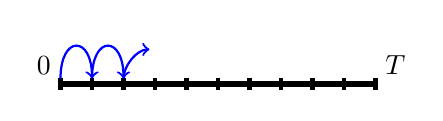
\begin{tikzpicture}[scale=0.8]
      \draw[color=black,line width=2.1](0.0,0.0) -- (5,0.0);
      %\draw[color=blue, line width=10] (0,-0.02) node {$\bullet$} ;
      %\draw[color=blue, line width=10] (5,-0.02) node {$\bullet$} ;
     % \draw node[color=blue,fill,circle,minimum size=0.01](1,1) {};
      \node[anchor=south east, color=black]
      at (0,0) {$0$};
      \node[anchor=south west, color=black]
      at (5,0) {$T$};
      
      \pgfmathsetmacro{\x}{0.0}
      \draw[color=black,line width=2.1](\x,0.1) -- (\x,-0.1);

      \pgfmathsetmacro{\x}{5.0}
      \draw[color=black,line width=2.1](\x,0.1) -- (\x,-0.1);

      \pgfmathsetmacro{\x}{0.5}
      \draw[color=black,line width=1.5](\x,0.1) -- (\x,-0.1);
      \draw[arrowStyle,color=blue]
      (\x-0.5,0) to[out=90,in=90,looseness=4.0]
      node[sloped,anchor=south]
      {}
      (\x,0.0);
      \draw[color=black,line width=1.5](\x,0.1) -- (\x,-0.1);


      
      \pgfmathsetmacro{\x}{1.0}
            \draw[arrowStyle,color=blue]
      (\x-0.5,0) to[out=90,in=90,looseness=4.0]
      node[sloped,anchor=south]
      {}
      (\x,0.0);
      \draw[color=black,line width=1.5](\x,0.1) -- (\x,-0.1);
      \pgfmathsetmacro{\x}{1.5}
            \draw[arrowStyle,color=blue]
      (\x-0.5,0) to[out=90,in=180,looseness=1.0]
      node[sloped,anchor=south]
      {}
      (\x,0.55);

      
      \draw[color=black,line width=1.5](\x,0.1) -- (\x,-0.1);
      \pgfmathsetmacro{\x}{2.0}
      \draw[color=black,line width=1.5](\x,0.1) -- (\x,-0.1);
      \pgfmathsetmacro{\x}{2.5}
      \draw[color=black,line width=1.5](\x,0.1) -- (\x,-0.1);
      \pgfmathsetmacro{\x}{3.0}
      \draw[color=black,line width=1.5](\x,0.1) -- (\x,-0.1);
      \pgfmathsetmacro{\x}{3.5}
      \draw[color=black,line width=1.5](\x,0.1) -- (\x,-0.1);
      \pgfmathsetmacro{\x}{4.0}
      \draw[color=black,line width=1.5](\x,0.1) -- (\x,-0.1);
      \pgfmathsetmacro{\x}{4.5}
      \draw[color=black,line width=1.5](\x,0.1) -- (\x,-0.1);
    \end{tikzpicture}

Time-steps going Forward
    \end{figure}
    \columnbreak
    \noindent
    \begin{empheq}[left=\empheqlbrace]{align}
   \boldsymbol{~~~}   & \frac{\partial \discreteLbd}{\partial t}^n=A\discreteLbd^n+R^*(R\discreteU^n-\textcolor{blue}{d_{obs}})\\
  & \text{With : ~~}  \discreteLbd^n=\vectll{(}{\discreteLbdun^n}{\discreteLbdeux^n}{)}
    \end{empheq}
    \vspace{-0.0cm}
    \noindent
    \begin{figure}
      \noindent
       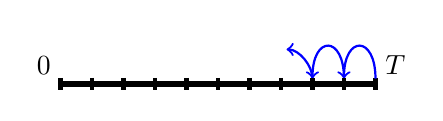
\begin{tikzpicture}[scale=0.8]
      \draw[color=black,line width=2.1](0.0,0.0) -- (5,0.0);
      %\draw[color=blue, line width=10] (0,-0.02) node {$\bullet$} ;
      %\draw[color=blue, line width=10] (5,-0.02) node {$\bullet$} ;
     % \draw node[color=blue,fill,circle,minimum size=0.01](1,1) {};
      \node[anchor=south east, color=black]
      at (0,0) {$0$};
      \node[anchor=south west, color=black]
      at (5,0) {$T$};
      
      \pgfmathsetmacro{\x}{0.0}
      \draw[color=black,line width=2.1](\x,0.1) -- (\x,-0.1);

      \pgfmathsetmacro{\x}{5.0}
      \draw[color=black,line width=2.1](\x,0.1) -- (\x,-0.1);

      \pgfmathsetmacro{\x}{0.5}
      \draw[color=black,line width=1.5](\x,0.1) -- (\x,-0.1);
      \draw[color=black,line width=1.5](\x,0.1) -- (\x,-0.1);


      
      \pgfmathsetmacro{\x}{1.0}
      \draw[color=black,line width=1.5](\x,0.1) -- (\x,-0.1);
      \pgfmathsetmacro{\x}{1.5}
      \draw[color=black,line width=1.5](\x,0.1) -- (\x,-0.1);
      \pgfmathsetmacro{\x}{2.0}
      \draw[color=black,line width=1.5](\x,0.1) -- (\x,-0.1);
      \pgfmathsetmacro{\x}{2.5}
      \draw[color=black,line width=1.5](\x,0.1) -- (\x,-0.1);
      \pgfmathsetmacro{\x}{3.0}
      \draw[color=black,line width=1.5](\x,0.1) -- (\x,-0.1);
      \pgfmathsetmacro{\x}{3.5}


      \draw[arrowStyle,color=blue]
      (\x+0.5,0) to[out=90,in=0,looseness=1.0]
      node[sloped,anchor=south]
      {}
      (\x,0.55);
      

      
      \draw[color=black,line width=1.5](\x,0.1) -- (\x,-0.1);
      \pgfmathsetmacro{\x}{4.0}


      \draw[arrowStyle,color=blue]
      (\x+0.5,0) to[out=90,in=90,looseness=4.0]
      node[sloped,anchor=south]
      {}
      (\x,0.0);
      
      
      \draw[color=black,line width=1.5](\x,0.1) -- (\x,-0.1);
      \pgfmathsetmacro{\x}{4.5}

      \draw[arrowStyle,color=blue]
      (\x+0.5,0) to[out=90,in=90,looseness=4.0]
      node[sloped,anchor=south]
      {}
      (\x,0.0);
      
      \draw[color=black,line width=1.5](\x,0.1) -- (\x,-0.1);
    \end{tikzpicture}

      Time-steps going Backward
    \end{figure}
  \end{multicols}
\end{frame}







\subsection{Discretize then Adjoint}

% ============================================
% ====== Frame : Discretize then Adjoint 1 ===
% ============================================
\begin{frame}{DtA : Discretize then Adjoint Strategy}{Example With RK4}

  All time scheme can be summed-up such as :
  \begin{equation}
    \textcolor{\myblue}{\boldsymbol{L}}\discreteU=\textcolor{\myblue}{\boldsymbol{E}}\discreteF
  \end{equation}

  \small
      RK4 time-scheme leads to :
    \begin{equation}
      \discreteU^{n+1}=B\discreteU^n+\textcolor{\myblue}{\boldsymbol{C_0}}\discreteF^n+\textcolor{\myblue}{\boldsymbol{C_{\frac{1}{2}}}}\discreteF^{n+\frac{1}{2}}+\textcolor{\myblue}{\boldsymbol{C_1}}\discreteF^{n+1}
    \end{equation}

\begin{equation}
  \textcolor{\myblue}{\boldsymbol{L}}\discreteU=\textcolor{\myblue}{\boldsymbol{E}}\discreteF=\discreteG
\end{equation}
\begin{equation}
  \begin{pmatrix}
    I & & & & \\
    -B&I & & & \\
    & -B&I  & & \\
    & & \ddots & \ddots   & \\
    & &  & -B &I \\
    %% \vdots & \ddots & \vdots \\
    %% 0      & \cdots & 1
  \end{pmatrix}
    \begin{pmatrix}
    \discreteU^0 \\
    \discreteU^1 \\
    \discreteU^2 \\
    \vdots \\
    \discreteU^n \\
  \end{pmatrix}=
  \begin{pmatrix}
    \discreteG^0 \\
    \discreteG^1 \\
    \discreteG^2 \\
    \vdots \\
    \discreteG^n \\
  \end{pmatrix}
  \end{equation}
\end{frame}



% ============================================
% ====== Frame : Discretize then Adjoint 2 ===
% ============================================
\begin{frame}{DtA : Discretize then Adjoint Strategy}

    All time scheme can be summed-up such as :
    \begin{equation}
      \textcolor{\myblue}{\boldsymbol{L}}\discreteU=\textcolor{\myblue}{\boldsymbol{E}}\discreteF \uncover<2->{=\discreteG}
    \end{equation}
    We are looking for a Discrete Adjoint state satisfying :
    \begin{equation}
      \textcolor{\myblue}{\boldsymbol{L^*}}\discreteLbd=-R^*(\textcolor{blue}{d_{obs}}-R\discreteU) \uncover<2->{=\discreteD}
    \end{equation}
    With the adjoint operator $\textcolor{\myblue}{\boldsymbol{L^*}}$ satisfying :
      \begin{equation}
    <\textcolor{\myblue}{\boldsymbol{L}}\discreteU,\discreteLbd>=<\discreteU,\textcolor{\myblue}{\boldsymbol{L^*}}\discreteLbd>
      \end{equation}
      \uncover<2->{
        \begin{equation}
        <\discreteG,\discreteLbd>=<\discreteU,\discreteD> \text{~~~(Adjoint Test)}
      \end{equation}


      \begin{center}
        Adjoint test succeeds $\Longleftrightarrow$  operator $\textcolor{\myblue}{\boldsymbol{L^*}}$  well established
      \end{center}
      }
\end{frame}




% ================================================
% ====== Frame : return on RK4 case ==============
% ================================================

\begin{frame}{DtA : Discretize then Adjoint Strategy}{Example with RK4}
\small
      RK4 time-scheme leads to :
    \begin{equation}
      \discreteU^{n+1}=B\discreteU^n+C_0\discreteF^n+C_{\frac{1}{2}}\discreteF^{n+\frac{1}{2}}+C_1\discreteF^{n+1}
    \end{equation}

\begin{equation}
  L\discreteU=E\discreteF=\discreteG
\end{equation}
\begin{equation}
  \begin{pmatrix}
    I & & & & \\
    -B&I & & & \\
    & -B&I  & & \\
    & & \ddots & \ddots   & \\
    & &  & -B &I \\
    %% \vdots & \ddots & \vdots \\
    %% 0      & \cdots & 1
  \end{pmatrix}
  \begin{pmatrix}
    \discreteU^0 \\
    \discreteU^1 \\
    \discreteU^2 \\
    \vdots \\
    \discreteU^n \\
  \end{pmatrix}=
  \begin{pmatrix}
    \discreteG^0 \\
    \discreteG^1 \\
    \discreteG^2 \\
    \vdots \\
    \discreteG^n \\
  \end{pmatrix}
\end{equation}

So :

\begin{equation}
  L^*=\begin{pmatrix}
  I &-B^* & & & \\
  &I &-B^* & & \\
  & &\ddots  &\ddots & \\
  & &  & I   &-B^* \\
  & &  &  &I \\
  %% \vdots & \ddots & \vdots \\
  %% 0      & \cdots & 1
  \end{pmatrix}
\end{equation}
\end{frame}





% ================================================
% ====== Frame : Adjoint Strategies Comparison ===
% ================================================

\begin{frame}{Adjoint Strategies Comparison}
  \begin{columns}
    \begin{column}[t]{0.5\textwidth}
      \textbf{\textcolor{red}{Adjoint Then Discretize}}
      \vspace{0.5cm}
%      \dotfill % to show column margins
      \begin{itemize}
      \item[\textcolor{\mygreen}{\textbf{+}}] Physical approach
      \item[\textcolor{\mygreen}{\textbf{+}}] Same discrete operators for Forward and Backward
      \item[\textbf{- -}] Inaccurate gradient \cite{Sirkes}
      \end{itemize}
      %      \dotfill
      \vspace{0.5cm}
    \end{column}\vrule \hfill
    \begin{column}[t]{0.5\textwidth}
      \textbf{\textcolor{blue}{Discretize then Adjoint}}
      \vspace{0.5cm}
%            \dotfill
      \begin{itemize}
      \item[\textcolor{\mygreen}{\textbf{+}}] Numerical approach
      \item[\textcolor{\mygreen}{\textbf{+}}] Has an Adjoint Test
      \item[\textbf{-}] Tremendous work to develop the adjoint operators
      \item[\textcolor{black}{\textbf{?}}] Non-consistency of the adjoint state \cite{Set1997Feb}
      \end{itemize}
    \end{column}
  \end{columns}

  \vfill
  \tiny
  \begin{thebibliography}{2}
    \bibitem{Sirkes} Sirkes, Ziv and Tziperman, Eli
      \newblock Finite Difference of Adjoint or Adjoint of Finite Difference ?
      \newblock 1997
  \bibitem{Set1997Feb} Sei Alain and Symes William
    \newblock A Note on Consistency and Adjointness for Numerical Schemes
    \newblock 1997
  \end{thebibliography}

\end{frame}
  %% AtD and DtA
%\tablesofcontent

\section{Some Results}
\subsection{1D Preliminary tests}
\begin{frame}{1D Preliminary tests}
    \begin{figure}
       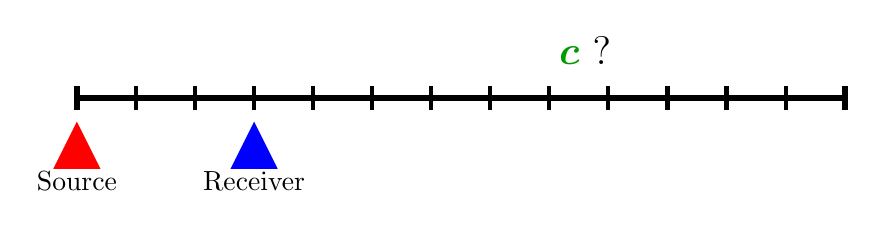
\begin{tikzpicture}[scale=1.5]
      \draw[color=black,line width=2.1](0.0,0.0) -- (6.5,0);
      %\draw[color=blue, line width=10] (0,-0.02) node {$\bullet$} ;
      %\draw[color=blue, line width=10] (5,-0.02) node {$\bullet$} ;
     % \draw node[color=blue,fill,circle,minimum size=0.01](1,1) {};
      \node[anchor=south east, color=black]
      at (0,0) {};
      \node[anchor=south west, color=black]
      at (4.0,0.2) {\Large $\velocity$ ?};

      \pgfmathsetmacro{\x}{0.0}
      \draw[color=black,line width=2.1](\x,0.1) -- (\x,-0.1);

      \pgfmathsetmacro{\x}{6.5}
      \draw[color=black,line width=2.1](\x,0.1) -- (\x,-0.1);

      \pgfmathsetmacro{\x}{0.5}
      \draw[color=black,line width=1.5](\x,0.1) -- (\x,-0.1);
      \draw[color=black,line width=1.5](\x,0.1) -- (\x,-0.1);



      \pgfmathsetmacro{\x}{1.0}
      \draw[color=black,line width=1.5](\x,0.1) -- (\x,-0.1);
      \pgfmathsetmacro{\x}{1.5}

      \draw[color=black,line width=1.5](\x,0.1) -- (\x,-0.1);
      \pgfmathsetmacro{\x}{2.0}
      \draw[color=black,line width=1.5](\x,0.1) -- (\x,-0.1);
      \pgfmathsetmacro{\x}{2.5}
      \draw[color=black,line width=1.5](\x,0.1) -- (\x,-0.1);
      \pgfmathsetmacro{\x}{3.0}
      \draw[color=black,line width=1.5](\x,0.1) -- (\x,-0.1);
      \pgfmathsetmacro{\x}{3.5}
      \draw[color=black,line width=1.5](\x,0.1) -- (\x,-0.1);
      \pgfmathsetmacro{\x}{4.0}
      \draw[color=black,line width=1.5](\x,0.1) -- (\x,-0.1);
      \pgfmathsetmacro{\x}{4.5}
      \draw[color=black,line width=1.5](\x,0.1) -- (\x,-0.1);
            \pgfmathsetmacro{\x}{5.0}
      \draw[color=black,line width=1.5](\x,0.1) -- (\x,-0.1);

            \pgfmathsetmacro{\x}{5.5}
      \draw[color=black,line width=1.5](\x,0.1) -- (\x,-0.1);


            \pgfmathsetmacro{\x}{6.0}
      \draw[color=black,line width=1.5](\x,0.1) -- (\x,-0.1);

      \pgfmathsetmacro{\x}{1.5}
      \pgfmathsetmacro{\dx}{0.2}
      \pgfmathsetmacro{\y}{-0.2}
      \pgfmathsetmacro{\dy}{-0.4}
      \node (A) at (\x,\y) {}; % B = 5
      \node (B) at (\x+\dx,\y+\dy) {}; % AC = 3
      \node (C) at (\x-\dx,\y+\dy) {}; % BC = 4
      \node (receiver) at (\x,\y+\dy-0.1) {Receiver}; % BC = 4
     % \draw (A) -- (B) -- (C) -- (A);
      \begin{scope}[on background layer]
        \fill [blue] (A.center) -- (B.center) -- (C.center) -- cycle;
      \end{scope}

            \pgfmathsetmacro{\x}{0.0}
      \pgfmathsetmacro{\dx}{0.2}
      \pgfmathsetmacro{\y}{-0.2}
      \pgfmathsetmacro{\dy}{-0.4}
      \node (A) at (\x,\y) {}; % B = 5
      \node (B) at (\x+\dx,\y+\dy) {}; % AC = 3
      \node (C) at (\x-\dx,\y+\dy) {}; % BC = 4
      \node (source) at (\x,\y+\dy-0.1) {Source}; % BC = 4
      %\draw [red] (A) -- (B) -- (C) -- (A);
      \begin{scope}[on background layer]
        \fill [red] (A.center) -- (B.center) -- (C.center) -- cycle;
      \end{scope}
\end{tikzpicture}

    \end{figure}

    \begin{multicols}{2}

      \begin{center}
        Initial $\velocity$ Model
      \end{center}
      \vspace{-0.1cm}

      \setlength{\plotwidth} {4.0cm}
      \setlength{\plotheight}{3cm}
      \begin{figure}
        \centering
          \begin{tikzpicture}
      \begin{axis}[%
          width=\plotwidth, height=\plotheight,,
          at={(0,0)},scale only axis,separate axis lines,xminorticks=true,
          xlabel={Depth},
          %ylabel={$\velocity$},
          %%   ymode=log,
          yminorticks=true,
          %xmin=0.,xmax=100.,
          ymin=0.98,ymax=1.22
        ]

        %% load current data
        %% -----------------
        \addplot[color=blue!50!black,mark options={solid},
          forget plot,line width=1pt,
          mark size=2pt]
        table[x=monx,y=mony]
        {images/VP0.dat};
        %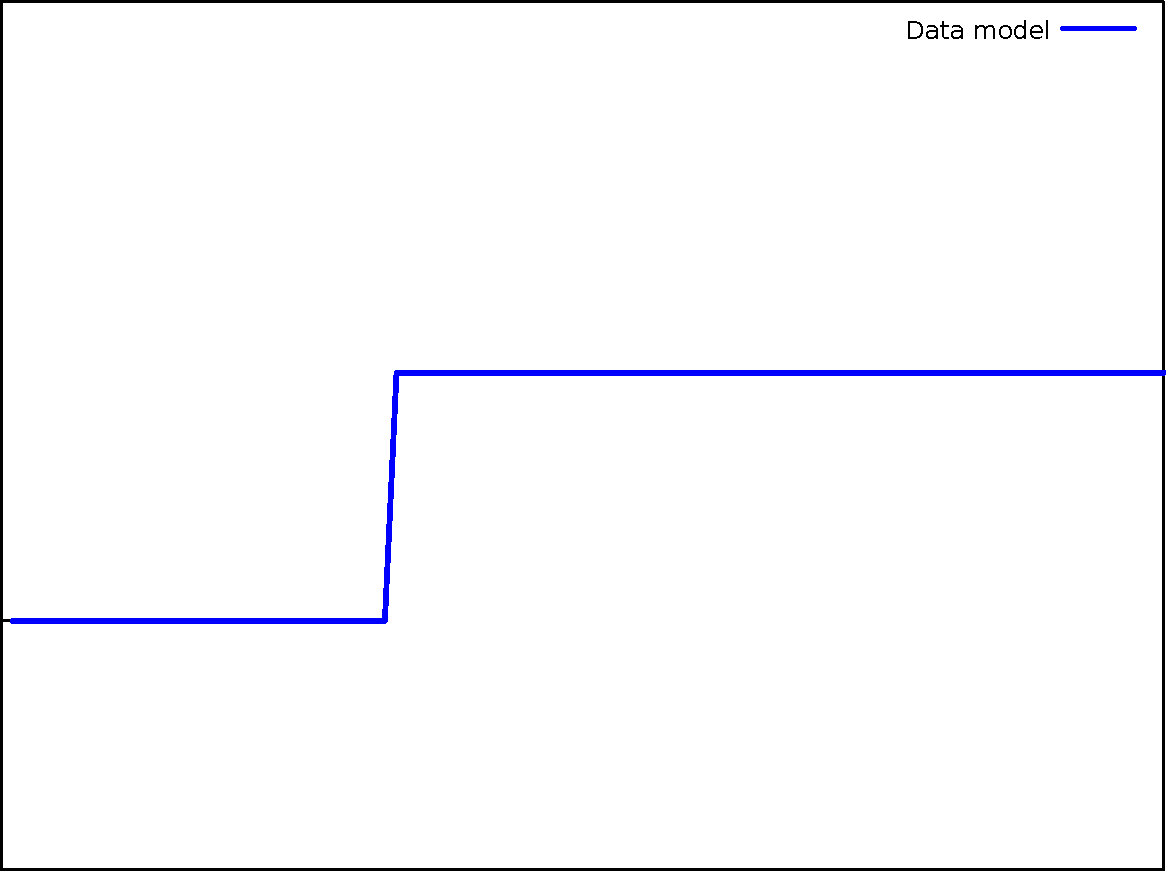
\includegraphics{images/data_bis.pdf}
      \end{axis}
      %% --------------------------------------------------------------------
          \end{tikzpicture}
          \end{figure}

      \columnbreak

      \begin{center}
        Target $\velocity$ Model
      \end{center}
      \vspace{-1.5cm}

      \begin{figure}
        \centering
          \begin{tikzpicture}
      \begin{axis}[%
          width=\plotwidth, height=\plotheight,,
          at={(0,0)},scale only axis,separate axis lines,xminorticks=true,
          xlabel={Depth},
          %ylabel={$\velocity$},
          %%   ymode=log,
          yminorticks=true,
          %%   xmin=0.,xmax=100.
        ]

        %% load current data
        %% -----------------
        \addplot[color=blue!50!black,mark options={solid},
          forget plot,line width=1pt,
          mark size=2pt]
        table[x=monx,y=mony]
        {images/VP100.dat};
      \end{axis}
      %% --------------------------------------------------------------------
          \end{tikzpicture}
          \end{figure}

      \end{multicols}

\end{frame}


%%%%%%%%%%%%%%%%%%%%%%%%%%%%%%%%%%%%%%%%%%%%% 1 %%%%%%%%%%%%%%%%%%%%%%%%%%%%%%%%%%%%%%%%%%%%%%%%
\begin{frame}{1D Preliminary tests :}
  \begin{multicols}{2}
    \normalsize
1D FWI :
\begin{itemize}
\item Lagrange / B-Bézier Operators
\item RK4 / AB3 time-schemes
\end{itemize}
\vspace{0.5cm}
\uncover<2->{
Adjoint test passed with :
\begin{itemize}
\item With a canonical space inner-product ($<u,v>_X=\sum_i u_iv_i$)
\item With a M-space inner product ($<u,v>_X^M=<Mu,v>_X$)
\end{itemize}}
\columnbreak
Gradient expression :
  \begin{equation}
     \nabla_{{\velocity}}\CF=-\int_0^{T} \int_{\Omega} \frac{2}{\density \velocity^3} \frac{\partial \contP}{\partial t}\Lbdun d\Omega dt
  \end{equation}
  \vspace{0.2cm}
  \\
  \tiny
  \uncover<2->{
\code{./run}\\
\code{----- Adjoint test -------}\\
\code{ inner product U/D   553123.57586755091    }\\
\code{ inner product G/Q   553123.57586756046    }\\
}
  %% ------------------------------------\\
  \uncover<3->{
\code{./run}\\
\code{----- Adjoint test -------}\\
\code{ inner product U/D  -75077.332007383695  }\\
\code{ inner product G/Q  -75077.332007386358  }\\
%------------------------------------\\
\code{./run}\\
\code{----- Adjoint test -------}\\
\code{ inner product U/D   125669.89223600870  }\\
\code{ inner product G/Q   125669.89223600952  }\\
}
%------------------------------------\\
\end{multicols}
\end{frame}
%%%%%%%%%%%%%%%%%%%%%%%%%%%%%%%%%%%%%%%%%%%%% 1 %%%%%%%%%%%%%%%%%%%%%%%%%%%%%%%%%%%%%%%%%%%%%%%%


%%%%%%%%%%%%%%%%%%%%%%%%%%%%%%%%%%%%%%%%%%%%% 2 %%%%%%%%%%%%%%%%%%%%%%%%%%%%%%%%%%%%%%%%%%%%%%%%
\begin{frame}{1D Velocity Model Reconstructions}
  \setlength{\plotwidth} {10.3cm}
  \setlength{\plotheight}{6cm}
  \begin{figure}
    \centering
    \begin{tikzpicture}

      \begin{axis}[width=\plotwidth,
                   height=\plotheight,
                   xlabel={Depth},
                   ylabel={$\velocity$},
                   legend pos=south east]
        \addplot[color=red!90!black,mark options={solid},
          line width=1pt,
          mark size=2pt]
        table[x=monx,y=mony]
        {images/VP_ATD.dat};
        \addlegendentry{Adjoint Then Discretize\footnote{With Bernstein-Bézier elements}}
        \addplot[color=blue!90!black,mark options={solid},
          line width=1pt,
          mark size=2pt]
        table[x=monx,y=mony]
        {images/VP_DTA.dat};
        \addlegendentry{Discretize Then Adjoint\footnote{With canonical scalar product}}
      \end{axis}
    \end{tikzpicture}
  \end{figure}
  \begin{center}
    $\velocity$ Model at the 100th FWI iteration
  \end{center}


\end{frame}


%%%%%%%%%%%%%%%%%%%%%%%%%%%%%%%%%%%%%%%%%%%%% 2 %%%%%%%%%%%%%%%%%%%%%%%%%%%%%%%%%%%%%%%%%%%%%%%%
\begin{frame}{1D Velocity Model Reconstructions}

  \begin{minipage}[top]{0.5\linewidth}
    With RK4 :
  \end{minipage}
  \begin{minipage}[top]{0.4\linewidth}
    ~~~~~~~~~~~~~~~ With AB3 :
  \end{minipage}
  \begin{minipage}[top]{0.5\linewidth}
    \setlength{\plotwidth} {6.0cm}
    \setlength{\plotheight}{5cm}
      \begin{figure}
        \begin{tikzpicture}
          \begin{axis}[width=\plotwidth,
              height=\plotheight,
              ymode = log,
              ylabel near ticks, yticklabel pos=right,
              xlabel={FWI Iterations},
              legend pos=north east]
            \addplot[color=red!90!black,mark options={solid},
              line width=1pt,
              mark size=2pt]
            table[x=monx,y=mony]
            {images/run_atd_rk4_bb.txt};
            \addlegendentry{AtD}
            \addplot[color=blue!90!black,mark options={solid},
              line width=1pt,
              mark size=2pt]
            table[x=monx,y=mony]
            {images/run_dta_rk4_bb.txt};
            \addlegendentry{DtA}
          \end{axis}
        \end{tikzpicture}
      \end{figure}
    \end{minipage}\hfill
    \begin{minipage}[top]{0.5\linewidth}
      \begin{figure}
        \begin{tikzpicture}
          \setlength{\plotwidth} {6.0cm}
          \setlength{\plotheight}{5cm}
          \begin{axis}[width=\plotwidth,
              height=\plotheight,
              xlabel={FWI Iterations},
              ymode = log,
              ylabel={log(Cost Function)},
%              ylabel style={rotate=-90},
              legend pos=north east]
            \addplot[color=red!90!black,mark options={solid},
              line width=1pt,
              mark size=2pt]
            table[x=monx,y=mony]
            {images/run_atd_ab3_bb.txt};
            \addlegendentry{AtD}
            \addplot[color=blue!90!black,mark options={solid},
              line width=1pt,
              mark size=2pt]
            table[x=monx,y=mony]
            {images/run_dta_ab3_bb.txt};
            \addlegendentry{DtA}
          \end{axis}
        \end{tikzpicture}
      \end{figure}
    \end{minipage}

    \uncover<2->{
    \begin{itemize}
      \item For RK4 scheme : Similar convergency
      \item For AB3 scheme : \textcolor{red}{AtD} is slighly better than \textcolor{blue}{DtA}
      \item The slope strongly depends on the optimizer -> Impossibilty to conclude
    \end{itemize}
    }

\end{frame}

%%%%%%%%%%%%%%%%%%%%%%%%%%%%%%%%%%%%%%%%%%%%%%%%%%%%%%%%%%%%%%%%%%%%%%%%
\subsection{2D Time Domain FWI Results}
\begin{frame}{2D Time Domain Reconstruction}

2D FWI :
\begin{itemize}
\item Developped in Total environnement (DIP\footnote{\url{http://dip.inria.fr/}})
\item Nodal Space Operators (Lagrangian/Jacobian)
\item Modal Space Operators (Bernstein-Bézier)
\item Runge Kutta 2/4 and Adams Bashforth time-schemes
\end{itemize}
\vspace{0.5cm}
Discretize Then Adjoint strategy not implemented :
\begin{itemize}
\item Tremendous task in a complex industrial code
\end{itemize}
%% \columnbreak
%% \uncover<2->{
%% Gradient expression :
%%   \begin{equation}
%%      \nabla_{{\velocity}}J=-\int_0^{T} \int_{\Omega} \frac{2}{\density \velocity^3} \frac{\partial \contP}{\partial t}\Lbdun d\Omega dt.
%%   \end{equation}
\end{frame}


\begin{frame}[noframenumbering]{2D Time Domain Reconstruction}

2D FWI :
\begin{itemize}
\item Developped in Total environnement (DIP\footnote{\url{http://dip.inria.fr/}})
\item Nodal Operators (Lagrangian/Jacobian)
\item Modal Operators (Bernstein-Bézier)
\item Runge Kutta 2/4 and Adams Bashforth time-schemes
\end{itemize}
\vspace{0.5cm}
 Gradient expression :
  \begin{equation}
     \nabla_{\boldsymbol{\textcolor{\mygreen}{\frac{1}{\kappa}}}}\CF=\int_0^{T} \int_{\Omega} \frac{\partial \contP}{\partial t}\Lbdun d\Omega dt \text{~~~~ with : } \boldsymbol{\textcolor{\mygreen}{\kappa}}=\density \velocity^2
  \end{equation}
   $\velocity$, $\density$ and  $\boldsymbol{\textcolor{\mygreen}{\kappa}}$  Constant per elements
\end{frame}

\newlength{\modelwidth}
\setlength{\modelwidth}{10.8cm}
\newcommand{\modeltitle}{Initial $\velocity$ Model}

\begin{frame}{2D Time Domain FWI Reconstructions}{Time-schemes comparison}
  \vspace{-0.5cm}
  \renewcommand{\modelfile}{fig/marmousi_noise_ini}
  \begin{figure}
       \begin{tikzpicture}
\pgfmathsetmacro{\xmin} {0.}
\pgfmathsetmacro{\xmax} {12.}
\pgfmathsetmacro{\zmin} {0.}
\pgfmathsetmacro{\zmax} {2.5}

\begin{axis}[%
title={\small{\modeltitle}},
width=1.0\modelwidth,
height=0.4\modelwidth,
axis on top, separate axis lines,
xmin=\xmin, xmax=\xmax, %xlabel={x (km)},
ymin=\zmin, ymax=\zmax, ylabel={depth (km)},
yticklabels={},xticklabels={},
y dir=reverse,
colormap/paraview, colorbar,
point meta min=1.5e-3, point meta max=5.5e-3,
colorbar/width=2.5mm,
]
\addplot [forget plot] graphics [xmin=\xmin,xmax=\xmax,ymin=\zmin,ymax=\zmax] {{\modelfile}.png};
\end{axis}
\end{tikzpicture}%
 \hfill
  \end{figure}
  \vspace{-1cm}
  \renewcommand{\modeltitle}{Target $\velocity$ Model}
  \renewcommand{\modelfile}{fig/marmousi_target}
  \begin{figure}
       \begin{tikzpicture}
\pgfmathsetmacro{\xmin} {0.}
\pgfmathsetmacro{\xmax} {12.}
\pgfmathsetmacro{\zmin} {0.}
\pgfmathsetmacro{\zmax} {2.5}

\begin{axis}[%
title={\small{\modeltitle}},
width=1.0\modelwidth,
height=0.4\modelwidth,
axis on top, separate axis lines,
xmin=\xmin, xmax=\xmax, %xlabel={x (km)},
ymin=\zmin, ymax=\zmax, ylabel={depth (km)},
yticklabels={},xticklabels={},
y dir=reverse,
colormap/paraview, colorbar,
point meta min=1.5e-3, point meta max=5.5e-3,
colorbar/width=2.5mm,
]
\addplot [forget plot] graphics [xmin=\xmin,xmax=\xmax,ymin=\zmin,ymax=\zmax] {{\modelfile}.png};
\end{axis}
\end{tikzpicture}%
 \hfill
   \end{figure}
\end{frame}

\begin{frame}[noframenumbering]{2D Time Domain FWI Reconstructions}{Time-schemes comparison}
  \vspace{-0.5cm}
  \renewcommand{\modelfile}{fig/marmousi_noise_rk2}
  \renewcommand{\modeltitle}{\textbf{\textcolor{red}{RK2}} Reconstructed $\velocity$ Model (30 iterations)}
  \begin{figure}
    \begin{tikzpicture}
\pgfmathsetmacro{\xmin} {0.}
\pgfmathsetmacro{\xmax} {12.}
\pgfmathsetmacro{\zmin} {0.}
\pgfmathsetmacro{\zmax} {2.5}

\begin{axis}[%
title={\small{\modeltitle}},
width=1.0\modelwidth,
height=0.4\modelwidth,
axis on top, separate axis lines,
xmin=\xmin, xmax=\xmax, %xlabel={x (km)},
ymin=\zmin, ymax=\zmax, ylabel={depth (km)},
yticklabels={},xticklabels={},
y dir=reverse,
colormap/paraview, colorbar,
point meta min=1.5e-3, point meta max=5.5e-3,
colorbar/width=2.5mm,
]
\addplot [forget plot] graphics [xmin=\xmin,xmax=\xmax,ymin=\zmin,ymax=\zmax] {{\modelfile}.png};
\end{axis}
\end{tikzpicture}%
 \hfill
  \end{figure}
  \vspace{-1cm}
  \renewcommand{\modeltitle}{Target $\velocity$ Model}
  \renewcommand{\modelfile}{fig/marmousi_target}
  \begin{figure}
    \begin{tikzpicture}
\pgfmathsetmacro{\xmin} {0.}
\pgfmathsetmacro{\xmax} {12.}
\pgfmathsetmacro{\zmin} {0.}
\pgfmathsetmacro{\zmax} {2.5}

\begin{axis}[%
title={\small{\modeltitle}},
width=1.0\modelwidth,
height=0.4\modelwidth,
axis on top, separate axis lines,
xmin=\xmin, xmax=\xmax, %xlabel={x (km)},
ymin=\zmin, ymax=\zmax, ylabel={depth (km)},
yticklabels={},xticklabels={},
y dir=reverse,
colormap/paraview, colorbar,
point meta min=1.5e-3, point meta max=5.5e-3,
colorbar/width=2.5mm,
]
\addplot [forget plot] graphics [xmin=\xmin,xmax=\xmax,ymin=\zmin,ymax=\zmax] {{\modelfile}.png};
\end{axis}
\end{tikzpicture}%
 \hfill
  \end{figure}
\end{frame}

\begin{frame}[noframenumbering]{2D Time Domain FWI Reconstructions}{Time-schemes comparison}
  \vspace{-0.5cm}
  \renewcommand{\modelfile}{fig/marmousi_noise_rk4_2}
  \renewcommand{\modeltitle}{\textbf{\textcolor{red}{RK4}} Reconstructed $\velocity$ Model (30 iterations)}
  \begin{figure}
    \begin{tikzpicture}
\pgfmathsetmacro{\xmin} {0.}
\pgfmathsetmacro{\xmax} {12.}
\pgfmathsetmacro{\zmin} {0.}
\pgfmathsetmacro{\zmax} {2.5}

\begin{axis}[%
title={\small{\modeltitle}},
width=1.0\modelwidth,
height=0.4\modelwidth,
axis on top, separate axis lines,
xmin=\xmin, xmax=\xmax, %xlabel={x (km)},
ymin=\zmin, ymax=\zmax, ylabel={depth (km)},
yticklabels={},xticklabels={},
y dir=reverse,
colormap/paraview, colorbar,
point meta min=1.5e-3, point meta max=5.5e-3,
colorbar/width=2.5mm,
]
\addplot [forget plot] graphics [xmin=\xmin,xmax=\xmax,ymin=\zmin,ymax=\zmax] {{\modelfile}.png};
\end{axis}
\end{tikzpicture}%
 \hfill
  \end{figure}
  \vspace{-1cm}
  \renewcommand{\modeltitle}{Target $\velocity$ Model}
  \renewcommand{\modelfile}{fig/marmousi_target}
  \begin{figure}
    \begin{tikzpicture}
\pgfmathsetmacro{\xmin} {0.}
\pgfmathsetmacro{\xmax} {12.}
\pgfmathsetmacro{\zmin} {0.}
\pgfmathsetmacro{\zmax} {2.5}

\begin{axis}[%
title={\small{\modeltitle}},
width=1.0\modelwidth,
height=0.4\modelwidth,
axis on top, separate axis lines,
xmin=\xmin, xmax=\xmax, %xlabel={x (km)},
ymin=\zmin, ymax=\zmax, ylabel={depth (km)},
yticklabels={},xticklabels={},
y dir=reverse,
colormap/paraview, colorbar,
point meta min=1.5e-3, point meta max=5.5e-3,
colorbar/width=2.5mm,
]
\addplot [forget plot] graphics [xmin=\xmin,xmax=\xmax,ymin=\zmin,ymax=\zmax] {{\modelfile}.png};
\end{axis}
\end{tikzpicture}%
 \hfill
  \end{figure}
\end{frame}


\begin{frame}[noframenumbering]{2D Time Domain FWI Reconstructions}{Time-schemes comparison}
  \vspace{-0.5cm}
  \renewcommand{\modelfile}{fig/marmousi_noise_ab3}
  \renewcommand{\modeltitle}{\textbf{\textcolor{red}{AB3}} Reconstructed $\velocity$ Model (30 iterations)}
  \begin{figure}
       \begin{tikzpicture}
\pgfmathsetmacro{\xmin} {0.}
\pgfmathsetmacro{\xmax} {12.}
\pgfmathsetmacro{\zmin} {0.}
\pgfmathsetmacro{\zmax} {2.5}

\begin{axis}[%
title={\small{\modeltitle}},
width=1.0\modelwidth,
height=0.4\modelwidth,
axis on top, separate axis lines,
xmin=\xmin, xmax=\xmax, %xlabel={x (km)},
ymin=\zmin, ymax=\zmax, ylabel={depth (km)},
yticklabels={},xticklabels={},
y dir=reverse,
colormap/paraview, colorbar,
point meta min=1.5e-3, point meta max=5.5e-3,
colorbar/width=2.5mm,
]
\addplot [forget plot] graphics [xmin=\xmin,xmax=\xmax,ymin=\zmin,ymax=\zmax] {{\modelfile}.png};
\end{axis}
\end{tikzpicture}%
 \hfill
  \end{figure}
  \vspace{-1cm}
  \renewcommand{\modeltitle}{Target $\velocity$ Model}
  \renewcommand{\modelfile}{fig/marmousi_target}
  \begin{figure}
       \begin{tikzpicture}
\pgfmathsetmacro{\xmin} {0.}
\pgfmathsetmacro{\xmax} {12.}
\pgfmathsetmacro{\zmin} {0.}
\pgfmathsetmacro{\zmax} {2.5}

\begin{axis}[%
title={\small{\modeltitle}},
width=1.0\modelwidth,
height=0.4\modelwidth,
axis on top, separate axis lines,
xmin=\xmin, xmax=\xmax, %xlabel={x (km)},
ymin=\zmin, ymax=\zmax, ylabel={depth (km)},
yticklabels={},xticklabels={},
y dir=reverse,
colormap/paraview, colorbar,
point meta min=1.5e-3, point meta max=5.5e-3,
colorbar/width=2.5mm,
]
\addplot [forget plot] graphics [xmin=\xmin,xmax=\xmax,ymin=\zmin,ymax=\zmax] {{\modelfile}.png};
\end{axis}
\end{tikzpicture}%
 \hfill
   \end{figure}
\end{frame}

\begin{frame}{2D Time Domain FWI Reconstructions}{Nodal/Modal Comparison}

  \begin{multicols}{2}
    \begin{itemize}
    \item 47k P1 elements
    \item Time Scheme : AB3
    \item Constant $\density$ model ($\density=1$)
    \item 19 sources / 181 Receivers
    \item 30 iterations
    \item 120 cores
    \item Nodal computation time : 5h10
    \item Modal computation time : 7h10$^{[1]}$
    \end{itemize}
    \columnbreak

    \setlength{\plotwidth} {6.0cm}
    \setlength{\plotheight}{5cm}
    Cost function evolution :
   \begin{figure}
        \begin{tikzpicture}
          \begin{axis}[width=\plotwidth,
              height=\plotheight,
%              ymode = log,
              xlabel={FWI Iterations},
              legend pos=north east]
            \addplot[color=red!90!black,mark options={solid},
              line width=1pt,
              mark size=2pt]
            table[x=monx,y=mony]
            {fig/run_ab3_lag.txt};
            \addlegendentry{Nodal}
            \addplot[mark=*,color=blue!90!black,mark options={scale=0.7},
              line width=0pt,
              mark size=2pt]
            table[x=monx,y=mony]
            {fig/run_ab3_lag.txt};
            \addlegendentry{Modal}
          \end{axis}
        \end{tikzpicture}
      \end{figure}
  \end{multicols}

  %% pour mettre en bas et en petit
  \vfill
  \tiny
  %%%%%%%%%%%%%%%%%%%%%%%%%%%%%%%%%%
  \begin{thebibliography}{1}
  \bibitem{chan2017gpu} Chan J. and Warburton T.
    \newblock GPU-Accelerated Bernstein Bézier Discontinuous Galerkin Methods for Wave Problems
    \newblock SIAM Journal on Scientific Computing 2017
  \end{thebibliography}

\end{frame}

\subsection{2D Multiscale Reconstruction}
\begin{frame}{2D Multiscale Reconstructions}{Reconstruction with an initial smooth model}
  \vspace{-0.5cm}
  \renewcommand{\modelfile}{fig/marmousi_filter_0}
  \renewcommand{\modeltitle}{Initial $\velocity$ Model}
  \begin{figure}
       \begin{tikzpicture}
\pgfmathsetmacro{\xmin} {0.}
\pgfmathsetmacro{\xmax} {12.}
\pgfmathsetmacro{\zmin} {0.}
\pgfmathsetmacro{\zmax} {2.5}

\begin{axis}[%
title={\small{\modeltitle}},
width=1.0\modelwidth,
height=0.4\modelwidth,
axis on top, separate axis lines,
xmin=\xmin, xmax=\xmax, %xlabel={x (km)},
ymin=\zmin, ymax=\zmax, ylabel={depth (km)},
yticklabels={},xticklabels={},
y dir=reverse,
colormap/paraview, colorbar,
point meta min=1.5e-3, point meta max=5.5e-3,
colorbar/width=2.5mm,
]
\addplot [forget plot] graphics [xmin=\xmin,xmax=\xmax,ymin=\zmin,ymax=\zmax] {{\modelfile}.png};
\end{axis}
\end{tikzpicture}%
 \hfill
  \end{figure}
  \vspace{-1cm}
  \renewcommand{\modeltitle}{Target $\velocity$ Model}
  \renewcommand{\modelfile}{fig/marmousi_target}
  \begin{figure}
       \begin{tikzpicture}
\pgfmathsetmacro{\xmin} {0.}
\pgfmathsetmacro{\xmax} {12.}
\pgfmathsetmacro{\zmin} {0.}
\pgfmathsetmacro{\zmax} {2.5}

\begin{axis}[%
title={\small{\modeltitle}},
width=1.0\modelwidth,
height=0.4\modelwidth,
axis on top, separate axis lines,
xmin=\xmin, xmax=\xmax, %xlabel={x (km)},
ymin=\zmin, ymax=\zmax, ylabel={depth (km)},
yticklabels={},xticklabels={},
y dir=reverse,
colormap/paraview, colorbar,
point meta min=1.5e-3, point meta max=5.5e-3,
colorbar/width=2.5mm,
]
\addplot [forget plot] graphics [xmin=\xmin,xmax=\xmax,ymin=\zmin,ymax=\zmax] {{\modelfile}.png};
\end{axis}
\end{tikzpicture}%
 \hfill
   \end{figure}
\end{frame}

\begin{frame}[noframenumbering]{2D Multiscale Reconstructions}{Reconstruction with an initial smooth model}
  \vspace{-0.5cm}
  \renewcommand{\modelfile}{fig/marmousi_nofilter}
  \renewcommand{\modeltitle}{Reconstructed model $\velocity$ Model (30 iterations AB3)}
  \begin{figure}
       \begin{tikzpicture}
\pgfmathsetmacro{\xmin} {0.}
\pgfmathsetmacro{\xmax} {12.}
\pgfmathsetmacro{\zmin} {0.}
\pgfmathsetmacro{\zmax} {2.5}

\begin{axis}[%
title={\small{\modeltitle}},
width=1.0\modelwidth,
height=0.4\modelwidth,
axis on top, separate axis lines,
xmin=\xmin, xmax=\xmax, %xlabel={x (km)},
ymin=\zmin, ymax=\zmax, ylabel={depth (km)},
yticklabels={},xticklabels={},
y dir=reverse,
colormap/paraview, colorbar,
point meta min=1.5e-3, point meta max=5.5e-3,
colorbar/width=2.5mm,
]
\addplot [forget plot] graphics [xmin=\xmin,xmax=\xmax,ymin=\zmin,ymax=\zmax] {{\modelfile}.png};
\end{axis}
\end{tikzpicture}%
 \hfill
  \end{figure}
  \vspace{-1cm}
  \renewcommand{\modeltitle}{Target $\velocity$ Model}
  \renewcommand{\modelfile}{fig/marmousi_target}
  \begin{figure}
       \begin{tikzpicture}
\pgfmathsetmacro{\xmin} {0.}
\pgfmathsetmacro{\xmax} {12.}
\pgfmathsetmacro{\zmin} {0.}
\pgfmathsetmacro{\zmax} {2.5}

\begin{axis}[%
title={\small{\modeltitle}},
width=1.0\modelwidth,
height=0.4\modelwidth,
axis on top, separate axis lines,
xmin=\xmin, xmax=\xmax, %xlabel={x (km)},
ymin=\zmin, ymax=\zmax, ylabel={depth (km)},
yticklabels={},xticklabels={},
y dir=reverse,
colormap/paraview, colorbar,
point meta min=1.5e-3, point meta max=5.5e-3,
colorbar/width=2.5mm,
]
\addplot [forget plot] graphics [xmin=\xmin,xmax=\xmax,ymin=\zmin,ymax=\zmax] {{\modelfile}.png};
\end{axis}
\end{tikzpicture}%
 \hfill
   \end{figure}
\end{frame}



\begin{frame}{2D Multiscale Reconstructions}{Multiscale Principle}


  \setlength{\plotwidth} {6.0cm}
  \setlength{\plotheight}{3cm}
  \begin{figure}
    \begin{tikzpicture}
      \begin{axis}[width=\plotwidth,
          height=\plotheight,
          %              ymode = log,
          xlabel={FWI Iterations},
          ymin=-5,ymax=29
        ]
        \addplot[color=red!90!black,mark options={solid},
          line width=1pt,
          mark size=2pt]
        table[x=monx,y=mony]
        {fig/file1.txt};
      \end{axis}
    \end{tikzpicture}
  \end{figure}

  \begin{figure}
    \begin{tikzpicture}
      \begin{axis}[width=\plotwidth,
          height=\plotheight,
          %              ymode = log,
          xlabel={FWI Iterations},
        ]
        \addplot[color=red!90!black,mark options={solid},
          line width=1pt,
          mark size=2pt]
        table[x=monx,y=mony]
        {fig/file2.txt};
      \end{axis}
    \end{tikzpicture}
  \end{figure}


  \begin{figure}
    \begin{tikzpicture}
      \begin{axis}[width=\plotwidth,
          height=\plotheight,
          %              ymode = log,
          xlabel={FWI Iterations},
        ]
        \addplot[color=red!90!black,mark options={solid},
          line width=1pt,
          mark size=2pt]
        table[x=monx,y=mony]
        {fig/file3.txt};
      \end{axis}
    \end{tikzpicture}
  \end{figure}

\end{frame}


\begin{frame}{2D Multiscale Reconstructions}{Reconstruction with an initial smooth model}
  \vspace{-0.5cm}
  \renewcommand{\modelfile}{fig/marmousi_filter_0}
  \renewcommand{\modeltitle}{Initial $\velocity$ Model}
  \begin{figure}
       \begin{tikzpicture}
\pgfmathsetmacro{\xmin} {0.}
\pgfmathsetmacro{\xmax} {12.}
\pgfmathsetmacro{\zmin} {0.}
\pgfmathsetmacro{\zmax} {2.5}

\begin{axis}[%
title={\small{\modeltitle}},
width=1.0\modelwidth,
height=0.4\modelwidth,
axis on top, separate axis lines,
xmin=\xmin, xmax=\xmax, %xlabel={x (km)},
ymin=\zmin, ymax=\zmax, ylabel={depth (km)},
yticklabels={},xticklabels={},
y dir=reverse,
colormap/paraview, colorbar,
point meta min=1.5e-3, point meta max=5.5e-3,
colorbar/width=2.5mm,
]
\addplot [forget plot] graphics [xmin=\xmin,xmax=\xmax,ymin=\zmin,ymax=\zmax] {{\modelfile}.png};
\end{axis}
\end{tikzpicture}%
 \hfill
  \end{figure}
  \vspace{-1cm}
  \renewcommand{\modeltitle}{Target $\velocity$ Model}
  \renewcommand{\modelfile}{fig/marmousi_target}
  \begin{figure}
       \begin{tikzpicture}
\pgfmathsetmacro{\xmin} {0.}
\pgfmathsetmacro{\xmax} {12.}
\pgfmathsetmacro{\zmin} {0.}
\pgfmathsetmacro{\zmax} {2.5}

\begin{axis}[%
title={\small{\modeltitle}},
width=1.0\modelwidth,
height=0.4\modelwidth,
axis on top, separate axis lines,
xmin=\xmin, xmax=\xmax, %xlabel={x (km)},
ymin=\zmin, ymax=\zmax, ylabel={depth (km)},
yticklabels={},xticklabels={},
y dir=reverse,
colormap/paraview, colorbar,
point meta min=1.5e-3, point meta max=5.5e-3,
colorbar/width=2.5mm,
]
\addplot [forget plot] graphics [xmin=\xmin,xmax=\xmax,ymin=\zmin,ymax=\zmax] {{\modelfile}.png};
\end{axis}
\end{tikzpicture}%
 \hfill
   \end{figure}
\end{frame}

\begin{frame}[noframenumbering]{2D Multiscale Reconstructions}{Reconstruction with an initial smooth model}
  \vspace{-0.5cm}
  \renewcommand{\modelfile}{fig/marmousi_filter_1}
  \renewcommand{\modeltitle}{Reconstructed $\velocity$ Model with \textcolor{red}{1.0-2.5Hz} filter}
  \begin{figure}
       \begin{tikzpicture}
\pgfmathsetmacro{\xmin} {0.}
\pgfmathsetmacro{\xmax} {12.}
\pgfmathsetmacro{\zmin} {0.}
\pgfmathsetmacro{\zmax} {2.5}

\begin{axis}[%
title={\small{\modeltitle}},
width=1.0\modelwidth,
height=0.4\modelwidth,
axis on top, separate axis lines,
xmin=\xmin, xmax=\xmax, %xlabel={x (km)},
ymin=\zmin, ymax=\zmax, ylabel={depth (km)},
yticklabels={},xticklabels={},
y dir=reverse,
colormap/paraview, colorbar,
point meta min=1.5e-3, point meta max=5.5e-3,
colorbar/width=2.5mm,
]
\addplot [forget plot] graphics [xmin=\xmin,xmax=\xmax,ymin=\zmin,ymax=\zmax] {{\modelfile}.png};
\end{axis}
\end{tikzpicture}%
 \hfill
  \end{figure}
  \vspace{-1cm}
  \renewcommand{\modeltitle}{Target $\velocity$ Model}
  \renewcommand{\modelfile}{fig/marmousi_target}
  \begin{figure}
       \begin{tikzpicture}
\pgfmathsetmacro{\xmin} {0.}
\pgfmathsetmacro{\xmax} {12.}
\pgfmathsetmacro{\zmin} {0.}
\pgfmathsetmacro{\zmax} {2.5}

\begin{axis}[%
title={\small{\modeltitle}},
width=1.0\modelwidth,
height=0.4\modelwidth,
axis on top, separate axis lines,
xmin=\xmin, xmax=\xmax, %xlabel={x (km)},
ymin=\zmin, ymax=\zmax, ylabel={depth (km)},
yticklabels={},xticklabels={},
y dir=reverse,
colormap/paraview, colorbar,
point meta min=1.5e-3, point meta max=5.5e-3,
colorbar/width=2.5mm,
]
\addplot [forget plot] graphics [xmin=\xmin,xmax=\xmax,ymin=\zmin,ymax=\zmax] {{\modelfile}.png};
\end{axis}
\end{tikzpicture}%
 \hfill
   \end{figure}
\end{frame}

\begin{frame}[noframenumbering]{2D Multiscale Reconstructions}{Reconstruction with an initial smooth model}
  \vspace{-0.5cm}
  \renewcommand{\modelfile}{fig/marmousi_filter_2}
  \renewcommand{\modeltitle}{Reconstructed $\velocity$ Model with \textcolor{red}{1.0-7.5Hz} filter}
  \begin{figure}
       \begin{tikzpicture}
\pgfmathsetmacro{\xmin} {0.}
\pgfmathsetmacro{\xmax} {12.}
\pgfmathsetmacro{\zmin} {0.}
\pgfmathsetmacro{\zmax} {2.5}

\begin{axis}[%
title={\small{\modeltitle}},
width=1.0\modelwidth,
height=0.4\modelwidth,
axis on top, separate axis lines,
xmin=\xmin, xmax=\xmax, %xlabel={x (km)},
ymin=\zmin, ymax=\zmax, ylabel={depth (km)},
yticklabels={},xticklabels={},
y dir=reverse,
colormap/paraview, colorbar,
point meta min=1.5e-3, point meta max=5.5e-3,
colorbar/width=2.5mm,
]
\addplot [forget plot] graphics [xmin=\xmin,xmax=\xmax,ymin=\zmin,ymax=\zmax] {{\modelfile}.png};
\end{axis}
\end{tikzpicture}%
 \hfill
  \end{figure}
  \vspace{-1cm}
  \renewcommand{\modeltitle}{Target $\velocity$ Model}
  \renewcommand{\modelfile}{fig/marmousi_target}
  \begin{figure}
       \begin{tikzpicture}
\pgfmathsetmacro{\xmin} {0.}
\pgfmathsetmacro{\xmax} {12.}
\pgfmathsetmacro{\zmin} {0.}
\pgfmathsetmacro{\zmax} {2.5}

\begin{axis}[%
title={\small{\modeltitle}},
width=1.0\modelwidth,
height=0.4\modelwidth,
axis on top, separate axis lines,
xmin=\xmin, xmax=\xmax, %xlabel={x (km)},
ymin=\zmin, ymax=\zmax, ylabel={depth (km)},
yticklabels={},xticklabels={},
y dir=reverse,
colormap/paraview, colorbar,
point meta min=1.5e-3, point meta max=5.5e-3,
colorbar/width=2.5mm,
]
\addplot [forget plot] graphics [xmin=\xmin,xmax=\xmax,ymin=\zmin,ymax=\zmax] {{\modelfile}.png};
\end{axis}
\end{tikzpicture}%
 \hfill
   \end{figure}
\end{frame}

\begin{frame}[noframenumbering]{2D Multiscale Reconstructions}{Reconstruction with an initial smooth model}
  \vspace{-0.5cm}
  \renewcommand{\modelfile}{fig/marmousi_filter_3}
  \renewcommand{\modeltitle}{Reconstructed $\velocity$ Model with \textcolor{red}{1.0-10Hz} filter}
  \begin{figure}
       \begin{tikzpicture}
\pgfmathsetmacro{\xmin} {0.}
\pgfmathsetmacro{\xmax} {12.}
\pgfmathsetmacro{\zmin} {0.}
\pgfmathsetmacro{\zmax} {2.5}

\begin{axis}[%
title={\small{\modeltitle}},
width=1.0\modelwidth,
height=0.4\modelwidth,
axis on top, separate axis lines,
xmin=\xmin, xmax=\xmax, %xlabel={x (km)},
ymin=\zmin, ymax=\zmax, ylabel={depth (km)},
yticklabels={},xticklabels={},
y dir=reverse,
colormap/paraview, colorbar,
point meta min=1.5e-3, point meta max=5.5e-3,
colorbar/width=2.5mm,
]
\addplot [forget plot] graphics [xmin=\xmin,xmax=\xmax,ymin=\zmin,ymax=\zmax] {{\modelfile}.png};
\end{axis}
\end{tikzpicture}%
 \hfill
  \end{figure}
  \vspace{-1cm}
  \renewcommand{\modeltitle}{Target $\velocity$ Model}
  \renewcommand{\modelfile}{fig/marmousi_target}
  \begin{figure}
       \begin{tikzpicture}
\pgfmathsetmacro{\xmin} {0.}
\pgfmathsetmacro{\xmax} {12.}
\pgfmathsetmacro{\zmin} {0.}
\pgfmathsetmacro{\zmax} {2.5}

\begin{axis}[%
title={\small{\modeltitle}},
width=1.0\modelwidth,
height=0.4\modelwidth,
axis on top, separate axis lines,
xmin=\xmin, xmax=\xmax, %xlabel={x (km)},
ymin=\zmin, ymax=\zmax, ylabel={depth (km)},
yticklabels={},xticklabels={},
y dir=reverse,
colormap/paraview, colorbar,
point meta min=1.5e-3, point meta max=5.5e-3,
colorbar/width=2.5mm,
]
\addplot [forget plot] graphics [xmin=\xmin,xmax=\xmax,ymin=\zmin,ymax=\zmax] {{\modelfile}.png};
\end{axis}
\end{tikzpicture}%
 \hfill
   \end{figure}
\end{frame}

\begin{frame}[noframenumbering]{2D Multiscale Reconstructions}{Reconstruction with an initial smooth model}
  \vspace{-0.5cm}
  \renewcommand{\modelfile}{fig/marmousi_filter_5}
  \renewcommand{\modeltitle}{Reconstructed $\velocity$ Model with \textcolor{red}{1.0-15Hz} filter}
  \begin{figure}
       \begin{tikzpicture}
\pgfmathsetmacro{\xmin} {0.}
\pgfmathsetmacro{\xmax} {12.}
\pgfmathsetmacro{\zmin} {0.}
\pgfmathsetmacro{\zmax} {2.5}

\begin{axis}[%
title={\small{\modeltitle}},
width=1.0\modelwidth,
height=0.4\modelwidth,
axis on top, separate axis lines,
xmin=\xmin, xmax=\xmax, %xlabel={x (km)},
ymin=\zmin, ymax=\zmax, ylabel={depth (km)},
yticklabels={},xticklabels={},
y dir=reverse,
colormap/paraview, colorbar,
point meta min=1.5e-3, point meta max=5.5e-3,
colorbar/width=2.5mm,
]
\addplot [forget plot] graphics [xmin=\xmin,xmax=\xmax,ymin=\zmin,ymax=\zmax] {{\modelfile}.png};
\end{axis}
\end{tikzpicture}%
 \hfill
  \end{figure}
  \vspace{-1cm}
  \renewcommand{\modeltitle}{Target $\velocity$ Model}
  \renewcommand{\modelfile}{fig/marmousi_target}
  \begin{figure}
       \begin{tikzpicture}
\pgfmathsetmacro{\xmin} {0.}
\pgfmathsetmacro{\xmax} {12.}
\pgfmathsetmacro{\zmin} {0.}
\pgfmathsetmacro{\zmax} {2.5}

\begin{axis}[%
title={\small{\modeltitle}},
width=1.0\modelwidth,
height=0.4\modelwidth,
axis on top, separate axis lines,
xmin=\xmin, xmax=\xmax, %xlabel={x (km)},
ymin=\zmin, ymax=\zmax, ylabel={depth (km)},
yticklabels={},xticklabels={},
y dir=reverse,
colormap/paraview, colorbar,
point meta min=1.5e-3, point meta max=5.5e-3,
colorbar/width=2.5mm,
]
\addplot [forget plot] graphics [xmin=\xmin,xmax=\xmax,ymin=\zmin,ymax=\zmax] {{\modelfile}.png};
\end{axis}
\end{tikzpicture}%
 \hfill
   \end{figure}
\end{frame}


\begin{frame}{2D Multiscale Reconstructions}

  \begin{multicols}{2}
    \begin{itemize}
    \item 47k P1 elements
    \item Time Scheme : AB3
    \item Constant $\density$ model ($\density=1$)
    \item 19 sources / 181 Receivers
    \item 120 cores
    \item Computation time : 17h
    \item Frequencies : \textcolor{red}{1-2.5Hz} \\ ~ \\ ~
    \end{itemize}
    \columnbreak

    \setlength{\plotwidth} {6.0cm}
    \setlength{\plotheight}{5cm}
    Cost function evolution :
    \begin{figure}
      \begin{tikzpicture}
        \begin{axis}[width=\plotwidth,
            height=\plotheight,
%            ymode = log,
            xlabel={FWI Iterations},
            xmin=-5.0, xmax=105.0,
            legend pos=south east]
          \addplot[color=red!90!black,mark options={solid},
            line width=1pt,
            mark size=2pt]
          table[x=monx,y=mony]
          {fig/run_marmousi_smooth.txt};
          \addlegendentry{$\CF(m)$}
        \end{axis}
      \end{tikzpicture}
    \end{figure}
  \end{multicols}
\end{frame}

\begin{frame}[noframenumbering]{2D Multiscale Reconstructions}

  \begin{multicols}{2}
    \begin{itemize}
    \item 47k P1 elements
    \item Time Scheme : AB3
    \item Constant $\density$ model ($\density=1$)
    \item 19 sources / 181 Receivers
    \item 120 cores
    \item Computation time : 17h
    \item Frequencies : 1-2.5Hz / \textcolor{red}{1-5Hz} \\ ~
    \end{itemize}
    \columnbreak

    \setlength{\plotwidth} {6.0cm}
    \setlength{\plotheight}{5cm}
    Cost function evolution :
    \begin{figure}
      \begin{tikzpicture}
        \begin{axis}[width=\plotwidth,
            height=\plotheight,
%            ymode = log,
            xlabel={FWI Iterations},
            xmin=-5.0, xmax=105.0,
            legend pos=south east]
          \addplot[color=red!90!black,mark options={solid},
            line width=1pt,
            mark size=2pt]
          table[x=monx,y=mony]
          {fig/run_marmousi_smooth_2.txt};
          \addlegendentry{$\CF(m)$}
        \end{axis}
      \end{tikzpicture}
    \end{figure}
  \end{multicols}
\end{frame}

\begin{frame}[noframenumbering]{2D Multiscale Reconstructions}

  \begin{multicols}{2}
    \begin{itemize}
    \item 47k P1 elements
    \item Time Scheme : AB3
    \item Constant $\density$ model ($\density=1$)
    \item 19 sources / 181 Receivers
    \item 120 cores
    \item Computation time : 17h
    \item Frequencies : 1-2.5Hz / 1-5Hz / \textcolor{red}{1-7.5Hz} \\ ~
    \end{itemize}
    \columnbreak

    \setlength{\plotwidth} {6.0cm}
    \setlength{\plotheight}{5cm}
    Cost function evolution :
    \begin{figure}
      \begin{tikzpicture}
        \begin{axis}[width=\plotwidth,
            height=\plotheight,
%            ymode = log,
            xlabel={FWI Iterations},
            xmin=-5.0, xmax=105.0,
            legend pos=south east]
          \addplot[color=red!90!black,mark options={solid},
            line width=1pt,
            mark size=2pt]
          table[x=monx,y=mony]
          {fig/run_marmousi_smooth_3.txt};
          \addlegendentry{$\CF(m)$}
        \end{axis}
      \end{tikzpicture}
    \end{figure}
  \end{multicols}
\end{frame}


\begin{frame}[noframenumbering]{2D Multiscale Reconstructions}

  \begin{multicols}{2}
    \begin{itemize}
    \item 47k P1 elements
    \item Time Scheme : AB3
    \item Constant $\density$ model ($\density=1$)
    \item 19 sources / 181 Receivers
    \item 120 cores
    \item Computation time : 17h
    \item Frequencies : 1-2.5Hz / 1-5Hz / 1-7.5Hz / \textcolor{red}{1-10Hz} \\ ~
    \end{itemize}
    \columnbreak

    \setlength{\plotwidth} {6.0cm}
    \setlength{\plotheight}{5cm}
    Cost function evolution :
    \begin{figure}
      \begin{tikzpicture}
        \begin{axis}[width=\plotwidth,
            height=\plotheight,
%            ymode = log,
            xlabel={FWI Iterations},
            xmin=-5.0, xmax=105.0,
            legend pos=south east]
          \addplot[color=red!90!black,mark options={solid},
            line width=1pt,
            mark size=2pt]
          table[x=monx,y=mony]
          {fig/run_marmousi_smooth_4.txt};
          \addlegendentry{$\CF(m)$}
        \end{axis}
      \end{tikzpicture}
    \end{figure}
  \end{multicols}
\end{frame}

\begin{frame}[noframenumbering]{2D Multiscale Reconstructions}

  \begin{multicols}{2}
    \begin{itemize}
    \item 47k P1 elements
    \item Time Scheme : AB3
    \item Constant $\density$ model ($\density=1$)
    \item 19 sources / 181 Receivers
    \item 120 cores
    \item Computation time : 17h
    \item Frequencies : 1-2.5Hz / 1-5Hz / 1-7.5Hz / 1-10Hz / \textcolor{red}{1-15Hz}
    \end{itemize}
    \columnbreak

    \setlength{\plotwidth} {6.0cm}
    \setlength{\plotheight}{5cm}
    Cost function evolution :
    \begin{figure}
      \begin{tikzpicture}
        \begin{axis}[width=\plotwidth,
            height=\plotheight,
%            ymode = log,
            xlabel={FWI Iterations},
            xmin=-5.0, xmax=105.0,
            legend pos=south east]
          \addplot[color=red!90!black,mark options={solid},
            line width=1pt,
            mark size=2pt]
          table[x=monx,y=mony]
          {fig/run_marmousi_smooth_5.txt};
          \addlegendentry{$\CF(m)$}
        \end{axis}
      \end{tikzpicture}
    \end{figure}
  \end{multicols}
\end{frame}

\begin{frame}{Conclusion}
conclusion
\end{frame}
  %% Some results


\end{document}
